\documentclass{SGGW-thesis}

\INZYNIERSKAtrue
\WZIMtrue

\title{Modularny system zadań logicznych zrealizowany w języku C++ dla mikrokontrolera ATmega328P}
\Etitle{Modular logic task system implemented in C++ language for the ATmega328P microcontroller}
\author{Stanisław Stankiewicz}
\date{2026}
\album{217442}
\thesis{Praca dyplomowa na kierunku:}
\course{Informatyka}
\promotor{dra\ inż.\ Artura Wilińskiego}
\pworkplace{Instytut Informatyki Technicznej\\Katedra Systemów Informatycznych}

\usepackage{hyperref}
\usepackage{xcolor}
\usepackage{float}
\usepackage{longtable}
\usepackage{listings}
\lstset{
basicstyle=\ttfamily\footnotesize,
keywordstyle=\color{blue}\bfseries,
stringstyle=\color{red},
commentstyle=\color{green!60!black},
numbers=left,
numberstyle=\tiny\color{gray},
stepnumber=1,
numbersep=10pt,
tabsize=4,
showspaces=false,
showstringspaces=false,
breaklines=true,
frame=single,
captionpos=b,
inputencoding=utf8,
extendedchars=true,
literate={ą}{{\k{a}}}1
{ć}{{\'c}}1
{ę}{{\k{e}}}1
{ł}{{\l{}}}1
{ń}{{\'n}}1
{ó}{{\'o}}1
{ś}{{\'s}}1
{ż}{{\.z}}1
{ź}{{\'z}}1
{Ą}{{\k{A}}}1
{Ć}{{\'C}}1
{Ę}{{\k{E}}}1
{Ł}{{\L{}}}1
{Ń}{{\'N}}1
{Ó}{{\'O}}1
{Ś}{{\'S}}1
{Ż}{{\.Z}}1
{Ź}{{\'Z}}1
}

% Automatyczne wsadzanie wszystkich bloków lstlisting w twardą, niełamliwą przestrzeń strony
\usepackage{etoolbox}
\BeforeBeginEnvironment{lstlisting}{\par\vspace{1.5em}\noindent\begin{minipage}{\linewidth}}
    \AfterEndEnvironment{lstlisting}{\end{minipage}\par\vspace{1.5em}}

\raggedbottom
\begin{document}

\maketitle
\statementpage

\abstractpage
{Tematem pracy jest zaprojektowanie i implementacja modułowego systemu interaktywnych zadań logicznych opartego na mikrokontrolerach ATmega328P. Projekt zakładał stworzenie systemu wbudowanego stymulującego współpracę grupy użytkowników rozwiązujących powiązane zagadki pod presją czasu. Architektura umożliwia dowolną konfigurację oraz łatwe rozszerzanie układu o kolejne niezależne moduły. Praca obejmuje fazę koncepcyjną, projektowanie sprzętowe, implementację protokołu komunikacyjnego I$^2$C oraz integrację oprogramowania w języku C++. Wyniki testów wskazują, że zaimplementowane podsystemy działają stabilnie, a przyjęta sieć Nadrzędny-Podrzędny (ang. \textit{Master-Slave}) zapewnia skalowalność środowiska.}
{modułowy system wbudowany, C++, I2C, ATmega328P, praca inżynierska, SGGW}
{Modular logic task system implemented in C++ language for the ATmega328P microcontroller}
{The subject of this thesis is the design and implementation of a modular system of interactive logic tasks based on ATmega328P microcontrollers. The project involved creating an embedded system that stimulates the cooperation of a group of users solving interrelated puzzles under time pressure. The system architecture was planned to allow for arbitrary configuration and easy expansion with additional independent modules. The thesis covers the conceptual phase, hardware design, implementation of a communication protocol based on the I$^2$C bus, and software integration in C++. Validation test results indicate that the implemented subsystems exhibit stable operation, and the adopted Master-Slave network ensures scalability of the environment.}
{embedded system, C++, I2C, ATmega328P, engineering thesis, WULS}

{
  % Spis treści może być złożony z pojedynczą interlinią, np. jeśli jedna linia wychodzi na następną stronę.
  % W przeciwnym razie spis treści wstawić bez powyższego rozkazu i klamry.
  \doublespacing
  \tableofcontents
}

\startchapterfromoddpage % niezależnie od długości spisu treści pierwszy rozdział zacznie się na nieparzystej stronie

\chapter{Wstęp}
Wraz z dynamicznym rozwojem systemów wbudowanych (ang. \textit{embedded systems}) oraz postępującą miniaturyzacją sprzętu elektronicznego, mikrokontrolery stały się powszechnie dostępne dla szerokiego grona inżynierów i konstruktorów. Narzędzia te pozwalają na projektowanie zaawansowanych, interaktywnych urządzeń fizycznych wymuszających na użytkowniku logiczne myślenie i szybkie podejmowanie decyzji. Istniejące na rynku rozwiązania komercyjne (wykorzystywane m.in. w pokojach zagadek typu \textit{escape room} lub w celach edukacyjno-szkoleniowych) rzadko oferują jednak otwartą i modularną architekturę opartą na tanich, 8-bitowych mikrokontrolerach ułożonych w skalowalnej sieci. Z tego powodu podjęto próbę konstrukcji autorskiej platformy.

\section{Cel i uzasadnienie pracy}
Głównym celem niniejszej pracy jest zaprojektowanie architektoniczne oraz wdrożenie fizycznego, modularnego systemu zadań logicznych. System ten wymusza jednoczesne rozwiązywanie różnorodnych procedur zadaniowych przez wielu uczestników przed upływem wyznaczonego zakresu czasu. Rozwiązanie opiera się na decentralizacji interfejsów wejścia oraz wspólnym nadzorze poprzez stację zarządzającą.

Wybór tematu podyktowany był chęcią weryfikacji zagadnień związanych z programowaniem 8-bitowych mikrokontrolerów rodziny AVR (szczególnie modelu ATmega328P \cite{atmega328p_datasheet}), integracją obwodów elektronicznych i implementacją protokołów komunikacyjnych działających asynchronicznie. Konstrukcja niezawodnego systemu czasu rzeczywistego (ang. \textit{Real-Time System}) stanowi złożone zagadnienie techniczne. Wymagało ono m.in. zbudowania warstwy transportowej opartej na magistrali I$^2$C w celu zapewnienia bezkolizyjnej synchronizacji danych pomiędzy jednostką nadrzędną (zarządzającą logiką gry) a niezależnymi węzłami wykonawczymi. Ze względu na specyfikę projektu, konieczna była optymalizacja kodu \texttt{C++} pod kątem małej dostępności pamięci operacyjnej SRAM (na układach ATmega328P wynosi ona zaledwie 2\,KB).

\section{Analiza istniejących rozwiązań}
Projektowany system czerpie inspirację z popularnej gry kooperacyjnej \textit{Keep Talking and Nobody Explodes}, w której gracze muszą wspólnie rozbroić bombę, komunikując się i rozwiązując zagadki logiczne. Na rynku istnieją również komercyjne platformy dla pokoi zagadek (np. \textit{Escape Room Master}), oferujące gotowe sterowniki i oprogramowanie. Jednak większość tych rozwiązań opiera się na drogich sterownikach PLC lub mikrokomputerach typu Raspberry Pi. Niniejsza praca udowadnia, że podobną funkcjonalność można osiągnąć przy użyciu znacznie tańszych i bardziej energooszczędnych 8-bitowych mikrokontrolerów, zachowując przy tym pełną modularność i łatwość rozbudowy.

Dodatkową wartością zaproponowanego rozwiązania jest połączenie kilku mechanizmów rzadko występujących łącznie w prostych systemach AVR: automatycznego wykrywania modułów na magistrali I$^2$C, globalnej deterministycznej konfiguracji scenariusza gry (\textit{seed}), propagacji liczby błędów do wszystkich węzłów oraz odpornej na przypadkowe wyzwolenie procedury restartu.

\section{Zakres pracy}
Niniejsza praca inżynierska obejmuje pełen cykl projektowy i programistyczny – od zaplanowania architektury systemu i opracowania algorytmiki oprogramowania, aż do ostatecznych testów stabilności. Wyszczególniony wykaz obszarów zadaniowych zrealizowanych w ramach niniejszej pracy obejmuje:
\begin{itemize}
  \item opracowanie koncepcji sprzętowej i programowej topologii rozproszonej typu \textit{Master-Slave}, wykorzystującej mikrokontrolery ATmega328P \cite{atmega328p_datasheet},
  \item wdrożenie biblioteki \texttt{ModuleComms} opartej na protokole I$^2$C, obsługującej automatyczne wykrywanie modułów na magistrali (tzw. skanowanie adresów),
  \item zaprogramowanie stacji \textit{Master}, odpowiedzialnej za odliczanie czasu przy użyciu wielozadaniowości asynchronicznej oraz odbieranie potwierdzeń wykonania zadań z modułów,
  \item zaprogramowanie w języku C++ modułów: arytmetycznego, labiryntu (wyświetlacz OLED), radiowego (interpretacja alfabetu Morse'a), sekwencyjnego oraz modułu z przełącznikiem dźwigniowym,
  \item optymalizację użycia pamięci SRAM poprzez wykorzystanie pamięci Flash (dyrektywa \texttt{PROGMEM}) do przechowywania danych statycznych,
  \item realizację testów z uwzględnieniem sprzętowej i programowej eliminacji drgań styków (ang. \textit{debouncing}).
\end{itemize}

\chapter{Narzędzia i użyte technologie}
W niniejszym rozdziale przedstawiono technologie, narzędzia oraz biblioteki wykorzystane w niniejszej pracy. Dla każdego komponentu opisano jego rolę oraz sposób wykorzystania. Realizacja pracy opierała się na sprawdzonych rozwiązaniach otwartoźródłowych (ang. \textit{open-source}), co pozwoliło skupić się na logice gry zamiast na tworzeniu sterowników od podstaw.

\section{Mikrokontroler ATmega328P}
ATmega328P \cite{atmega328p_datasheet} to 8-bitowy mikrokontroler z rodziny AVR, posiadający 32\,KB pamięci programu (Flash), 2\,KB pamięci operacyjnej (SRAM) oraz 1\,KB pamięci danych (EEPROM). Dzięki architekturze RISC większość instrukcji wykonuje w jednym cyklu zegara, co zapewnia dobrą wydajność przy niskim poborze energii.

Wybór tego układu podyktowany był trzema czynnikami. Po pierwsze, stanowi on fundament popularnej platformy Arduino Uno, co daje dostęp do bardzo dużej liczby bibliotek oraz materiałów edukacyjnych. Po drugie, oferuje natywną obsługę peryferiów pracujących w standardzie 5\,V, co eliminuje potrzebę stosowania konwerterów napięć. Po trzecie, posiada sprzętowy kontroler I$^2$C (TWI), który jest fundamentem komunikacji w tym systemie.

W niniejszej pracy układy pracują pod kontrolą wewnętrznego oscylatora RC skonfigurowanego na częstotliwość 8\,MHz. Wykorzystanie wbudowanego źródła sygnału zegarowego, zamiast zewnętrznego rezonatora kwarcowego dostarczającego sygnał taktujący, obniża złożoność i koszt obwodu, a jednocześnie pozwala na pracę w poszerzonym zakresie napięć zasilania od 2.7\,V do 5.5\,V. Choć wbudowany oscylator charakteryzuje się tolerancją wahań do $\pm10\%$ (w stałych warunkach pokojowych błąd oscyluje w granicach $\pm$1--2\%), odchylenia te są pomijalne w kontekście działania gry oraz obsługi magistrali I$^2$C. Konfigurację niskopoziomową mikrokontrolera (ustawienie bitów konfiguracyjnych (ang. \textit{fuse bits}), odpowiedzialnych za trwałe ustawienia sprzętowe układu) przeprowadzono bezpośrednio przy użyciu narzędzia wiersza poleceń \texttt{avrdude}, co umożliwiło precyzyjne sterowanie parametrami pracy układu bez użycia dodatkowych nakładek systemowych. Bezpośrednie wgrywanie oprogramowania przez złącze programowania wewnątrzsystemowego (ang. \textit{In-System Programming} --- ISP) pozwoliło całkowicie wyeliminować program rozruchowy (ang. \textit{bootloader}), dzięki czemu kod programu ma do dyspozycji pełne 32\,KB pamięci Flash. Jest to istotna optymalizacja względem standardowej platformy Arduino Uno, w której część pamięci programu stale zajmuje wspomniany program rozruchowy.

\section{Środowisko Arduino IDE}
Arduino IDE \cite{cpp_arduino_ref} to środowisko programistyczne ułatwiające tworzenie oprogramowania na mikrokontrolery. Pozwala na pisanie kodu w C++ z wykorzystaniem gotowych bibliotek obsługujących m.in. przerwania czy komunikację.

Wybór Arduino IDE, zamiast alternatyw takich jak PlatformIO czy Atmel Studio, podyktowany był przede wszystkim dojrzałością ekosystemu bibliotek kompatybilnych z platformą AVR oraz niskim progiem wejścia przy prototypowaniu. Choć PlatformIO oferuje bardziej zaawansowane zarządzanie zależnościami, Arduino IDE zapewniło wystarczającą funkcjonalność przy jednocześniejszej prostocie konfiguracji wielomodułowego projektu.

W ramach niniejszej pracy proces programowania układów realizowano za pośrednictwem wspomnianego wcześniej narzędzia \texttt{avrdude} oraz zewnętrznego programatora sprzętowego USBasp. Na potrzeby seryjnego przygotowania mikrokontrolerów opracowano dedykowany adapter wyposażony w gniazdo typu ZIF (ang. \textit{Zero Insertion Force}) z mechanizmem dźwigniowym. Rozwiązanie to umożliwiło szybką i bezpieczną wymianę układów brzegowych bez ryzyka uszkodzenia ich wyprowadzeń, zapewniając stabilne połączenie z programatorem.

\section{Biblioteka komunikacji I$^2$C -- Wire.h}
Wire.h \cite{arduino_wire} jest standardową biblioteką środowiska Arduino, realizującą obsługę protokołu I$^2$C (\textit{Inter-Integrated Circuit}) za pośrednictwem wbudowanego sprzętowego kontrolera TWI mikrokontrolera ATmega328P. Biblioteka przejmuje zarządzanie rejestrami taktowania przesyłu, przerwaniami oraz identyfikacją sprzętową sygnałów potwierdzających komunikację (ACK/NACK).

Protokół I$^2$C został wybrany jako magistrala komunikacyjna systemu ze względu na minimalizację liczby wymaganych połączeń sygnałowych --- do połączenia dowolnej liczby urządzeń wystarczają zaledwie dwie linie sygnałowe (SDA i SCL) oraz wspólne zasilanie. W porównaniu z alternatywami, takimi jak SPI (wymagający dodatkowej linii CS dla każdego urządzenia) czy UART, I$^2$C stanowi optymalny kompromis między prostotą połączeń a skalowalnością. Co istotne, protokół UART jest interfejsem asynchronicznym, co przy braku zewnętrznego oscylatora kwarcowego i pracy na wewnętrznym oscylatorze RC mogłoby prowadzić do błędów synchronizacji ramek przy wahaniach temperatury. Magistrala I$^2$C, jako interfejs synchroniczny (wykorzystujący linię zegarową SCL), jest niewrażliwa na niedokładności taktowania mikrokontrolerów.

W niniejszej pracy biblioteka \texttt{Wire.h} stanowi fundament autorskiej biblioteki \texttt{ModuleComms}, realizując fizyczną warstwę transportową komunikacji między jednostką Master a modułami Slave.

\section{Biblioteki graficzne Adafruit}
Rodzina bibliotek Adafruit obejmuje \texttt{Adafruit\_GFX} \cite{Adafruit-GFX-Library} --- uniwersalny rdzeń graficzny 2D --- oraz \texttt{Adafruit\_SH110X} \cite{Adafruit_sh1106x} --- dedykowany sterownik dla wyświetlaczy OLED opartych na układzie SH1106G.

Biblioteki te wybrano ze względu na ich szeroką kompatybilność z ekosystemem Arduino, aktywne wsparcie społeczności oraz zoptymalizowane algorytmy rysowania, dostosowane do ograniczeń pamięciowych mikrokontrolerów 8-bitowych. Alternatywna biblioteka \texttt{U8g2lib}, choć oferuje podobną funkcjonalność, wykazuje większe zapotrzebowanie na pamięć SRAM, co stanowi istotne ograniczenie na platformie ATmega328P dysponującej zaledwie 2\,KB tego zasobu.

W niniejszej pracy biblioteki Adafruit wykorzystano w modułach labiryntu oraz radiowym do obsługi monochromatycznych wyświetlaczy OLED o rozdzielczości 128x64 pikseli. Warstwa \texttt{Adafruit\_GFX} umożliwia rysowanie prymitywów graficznych (prostokątów, okręgów, glifów tekstowych) oraz renderowanie bitmap przechowywanych w pamięci Flash za pośrednictwem dyrektywy \texttt{PROGMEM}, co pozwala na obsługę dużych zasobów graficznych bez obciążania ograniczonej pamięci SRAM.

\section{Biblioteka wyświetlacza LiquidCrystal}
Biblioteka \texttt{LiquidCrystal} \cite{arduino_liquid_crystal} jest standardowym narzędziem środowiska Arduino służącym do obsługi wyświetlaczy alfanumerycznych opartych na sterowniku Hitachi HD44780. Pozwala ona na komunikację z panelem LCD w trybie 4-bitowym lub 8-bitowym, co umożliwia elastyczne zarządzanie zasobami sprzętowymi mikrokontrolera.

W niniejszej pracy wykorzystano tryb 4-bitowy, który wymaga podłączenia sześciu linii sygnałowych (RS, EN oraz cztery linie danych). Choć rozwiązanie to zajmuje więcej pinów mikrokontrolera niż alternatywne interfejsy szeregowe, zapewnia ono najwyższą wydajność odświeżania oraz pełną kompatybilność z podstawowymi bibliotekami bez konieczności stosowania dodatkowych układów pośredniczących, takich jak ekspandery I$^2$C. Wybór ten był możliwy dzięki rezygnacji z innych peryferiów w module arytmetycznym (klawiaturze), co pozostawiło wystarczającą liczbę wolnych wyprowadzeń ATmega328P. W ramach niniejszej pracy biblioteka służy do wyświetlania treści zadań matematycznych oraz wprowadzanych przez użytkownika odpowiedzi na panelu LCD 16x2.

\section{Biblioteka TM1637Display}
TM1637Display \cite{TM1637Display} jest biblioteką obsługującą sprzętowy sterownik TM1637, stosowany w poczwórnych wyświetlaczach 7-segmentowych. Sterownik ten wykorzystuje dwuprzewodowy protokół komunikacyjny zbliżony koncepcyjnie do I$^2$C, lecz wymagający dedykowanych linii CLK i DIO.

Decyzja o zastosowaniu wyświetlacza TM1637 w jednostce nadrzędnej, zamiast np. wyświetlacza OLED, podyktowana była niskim kosztem komponentu, doskonałą czytelnością dużych cyfr z dalszej odległości oraz minimalnym zapotrzebowaniem na zasoby mikrokontrolera. Biblioteka realizuje transmisję danych bez stosowania blokujących opóźnień typu \texttt{delay()}, co jest kluczowe dla zachowania ciągłości asynchronicznego nasłuchu na magistrali I$^2$C w pętli głównej programu.

W niniejszej pracy wyświetlacz TM1637 pełni rolę głównego wskaźnika upływającego czasu gry w formacie MM:SS, informując uczestników o zbliżającym się jego końcu.

\section{Biblioteka interfejsu SPI}
SPI.h jest standardową biblioteką środowiska Arduino, realizującą obsługę protokołu \textit{Serial Peripheral Interface} (SPI). Interfejs ten umożliwia szybką, synchroniczną komunikację szeregową z peryferiami za pośrednictwem czterech linii sygnałowych: MOSI (\textit{Master Out Slave In}), MISO (\textit{Master In Slave Out}), SCK (\textit{Serial Clock}) oraz CS (\textit{Chip Select}).

Protokół SPI został zastosowany w module labiryntu zamiast I$^2$C z dwóch kluczowych powodów. Po pierwsze, magistrala SPI oferuje znacząco wyższą przepustowość, niezbędną do wydajnego przesyłania pełnych buforów ramki obrazu (1\,KB) do wyświetlacza OLED bez blokowania pętli głównej. Po drugie, mikrokontrolery ATmega328P posiadają tylko jeden sprzętowy interfejs I$^2$C, który w tym module jest już wykorzystywany do pracy w trybie Slave na potrzeby komunikacji systemowej. Jednoczesna obsługa wyświetlacza jako Master na tej samej magistrali byłaby programowo i sprzętowo nieefektywna, wymagając ciągłego i ryzykownego przełączania trybów pracy kontrolera TWI.

\chapter{Projekt systemu}
W niniejszym rozdziale przedstawiono projekt modularnego systemu zadań logicznych. Głównym celem projektu było opracowanie skalowalnej i łatwej w rozszerzaniu platformy sprzętowo-programowej, umożliwiającej jednoczesną, interaktywną pracę wielu uczestników z niezależnymi modułami zagadek, koordynowanymi przez centralną jednostkę zarządzającą. W kolejnych podrozdziałach szczegółowo opisano specyfikację wymagań, architekturę systemu oraz strukturę klas obiektowych.

\section{Specyfikacja wymagań}
Kluczowym etapem projektu jest określenie wymagań, które system musi spełniać. Na podstawie analizy problemu, przeglądu podobnych rozwiązań (np. w pokojach zagadek typu \textit{escape room}) oraz ograniczeń mikrokontrolerów AVR, wyodrębniono wymagania funkcjonalne i niefunkcjonalne.

\subsection{Wymagania funkcjonalne}
Wymagania funkcjonalne definiują zakres operacji i możliwości, które system musi dostarczyć użytkownikowi końcowemu. Kluczowe funkcje realizowane przez projektowany system zostały zestawione w Tabeli~\ref{tab:wymagania_funkcjonalne}.

\begin{longtable}{|c|p{3.8cm}|p{8.2cm}|}
  \caption{Wymagania funkcjonalne systemu} \label{tab:wymagania_funkcjonalne}                                                                                                                                       \\
  \hline
  \textbf{Numer} & \textbf{Nazwa}                       & \textbf{Opis}                                                                                                                                             \\
  \hline
  \endfirsthead

  \multicolumn{3}{c}%
  {{\bfseries Tabela \thetable{} -- kontynuacja z poprzedniej strony}}                                                                                                                                              \\
  \hline
  \textbf{Numer} & \textbf{Nazwa}                       & \textbf{Opis}                                                                                                                                             \\
  \hline
  \endhead

  \hline \multicolumn{3}{|r|}{{Kontynuacja na następnej stronie}}                                                                                                                                                   \\ \hline
  \endfoot

  \hline
  \endlastfoot

  WF-01          & Koordynacja czasu rozgrywki          & Centralny węzeł Master zarządza odliczaniem czasu dla wszystkich modułów. Błędy popełniane przez graczy powodują przyspieszenie odliczania czasu.         \\
  \hline
  WF-02          & Niezależna logika modułów zagadek    & Wszystkie obwody posiadają niezależny algorytm rozwiązywania, podlegając asynchronicznej komunikacji wymuszanej wyłącznie na prośbę węzła głównego.       \\
  \hline
  WF-03          & Determinizm konfiguracji (Seed)      & System inicjuje przed startem dystrybucję globalnego numeru konfiguracji po łączu I$^2$C, determinizując pseudolosowe zdarzenia we wszystkich układach.   \\
  \hline
  WF-04          & Obsługa wielu typów modułów          & System obsługuje co najmniej pięć typów modułów: arytmetyczny, labiryntu, radiowy, sekwencyjny oraz z przełącznikiem.                                     \\
  \hline
  WF-05          & Detekcja i propagacja błędów         & Niepoprawne działanie operatora generuje zdarzenie błędu rejestrowane globalnie przez Master. Akumulacja błędów wpływa na zachowanie pozostałych modułów. \\
  \hline
  WF-06          & Automatyczne wykrywanie topologii    & Serwer Master po uruchomieniu skanuje adresy magistrali I$^2$C w celu automatycznej identyfikacji podłączonych modułów bez ręcznej konfiguracji.          \\
  \hline
  WF-07          & Sygnalizacja dźwiękowa i~wizualna    & System zapewnia eskalujące ostrzeżenia dźwiękowe oraz wizualne informujące o zbliżającym się końcu limitu czasowego oraz o stanie błędu.                  \\
  \hline
  WF-08          & Mechanizm restartu z~zabezpieczeniem & Restart gry wymaga trzykrotnej aktywacji przełącznika w ustalonym oknie czasowym, zapobiegając przypadkowemu zresetowaniu rozgrywki.                      \\
  \hline
\end{longtable}

Zdefiniowane wymagania kładą nacisk na samodzielność modułów przy centralnej koordynacji. Obejmują one mechanizmy zarządzania rozgrywką (odliczanie czasu, błędy) oraz funkcje systemowe, takie jak automatyczne wykrywanie modułów czy konfiguracja gry za pomocą ziarna (ang. \textit{seed}).

\subsection{Wymagania niefunkcjonalne}
Wymagania niefunkcjonalne definiują cechy jakościowe systemu oraz techniczne ograniczenia projektu. Kluczowe wymagania z tej kategorii zestawiono w Tabeli~\ref{tab:wymagania_niefunkcjonalne}.

\begin{longtable}{|c|p{3.8cm}|p{8.2cm}|}
  \caption{Wymagania niefunkcjonalne systemu} \label{tab:wymagania_niefunkcjonalne}                                                                                                                                                           \\
  \hline
  \textbf{Numer} & \textbf{Nazwa}                        & \textbf{Opis}                                                                                                                                                                      \\
  \hline
  \endfirsthead

  \multicolumn{3}{c}%
  {{\bfseries Tabela \thetable{} -- kontynuacja z poprzedniej strony}}                                                                                                                                                                        \\
  \hline
  \textbf{Numer} & \textbf{Nazwa}                        & \textbf{Opis}                                                                                                                                                                      \\
  \hline
  \endhead

  \hline \multicolumn{3}{|r|}{{Kontynuacja na następnej stronie}}                                                                                                                                                                             \\ \hline
  \endfoot

  \hline
  \endlastfoot

  WN-01          & Modularność sprzętowa (Plug-and-Play) & Stacje podłączane są do wspólnej szyny I$^2$C na współdzielonym zasilaniu (+5\,V i GND), minimalizując liczbę styków montażowych z utrzymaniem odporności na przerwanie łączności. \\
  \hline
  WN-02          & Wielozadaniowość nieblokująca         & Zrezygnowanie z wywołań \texttt{delay()} w logice rdzeniowej. Ewaluacje stanów opierają się o mechanizm obliczeń delty z systemowego stopera \texttt{millis()}.                    \\
  \hline
  WN-03          & Efektywne wykorzystanie pamięci       & System funkcjonuje w ramach limitów ATmega328P (2\,KB SRAM, 32\,KB Flash). Duże struktury danych alokowane są w pamięci Flash za pośrednictwem \texttt{PROGMEM}.                   \\
  \hline
  WN-04          & Skalowalność                          & Architektura umożliwia rozszerzenie o dodatkowe moduły bez modyfikacji oprogramowania Master (do 126 urządzeń na magistrali I$^2$C).                                               \\
  \hline
  WN-05          & Niezawodność komunikacji              & Protokół transportowy jest odporny na chwilowe zaniki łączności z pojedynczymi modułami bez destabilizacji pracy pozostałych węzłów.                                               \\
  \hline
  WN-06          & Koszt i dostępność komponentów        & Projekt bazuje na tanich, powszechnie dostępnych komponentach elektronicznych w celu ograniczenia kosztów produkcji prototypu.                                                     \\
  \hline
  WN-07          & Stabilność zasilania                  & System funkcjonuje w zakresie napięć 2.7--5.5\,V, wykorzystując wewnętrzny oscylator RC 8\,MHz z tolerancją wahań $\pm$1--2\%.                                                     \\
  \hline
\end{longtable}

Wymagania te stawiają priorytet na wielozadaniowość oraz optymalizację pamięci --- co jest krytyczne przy zaledwie 2\,KB pamięci SRAM. Istotna jest także modularność typu Plug-and-Play, pozwalająca na dowolne podłączanie modułów bez zmian w oprogramowaniu sterownika głównego.

\section{Architektura systemu}
System oparto na architekturze nadrzędno-podrzędnej (ang. \textit{Master-Slave}), gdzie centralna jednostka koordynuje pracę modułów przez magistralę I$^2$C (\textit{Inter-Integrated Circuit}). Jest to szeregowy interfejs komunikacyjny wykorzystujący dwie linie sygnałowe: SDA (\textit{Serial Data}) do przesyłu danych oraz SCL (\textit{Serial Clock}) do synchronizacji zegarowej. Wybór tej magistrali podyktowany był jej oszczędnością w liczbie wymaganych połączeń oraz natywnym wsparciem przez sprzętowy kontroler TWI (\textit{Two Wire Interface}) mikrokontrolera ATmega328P \cite{atmega328p_datasheet}. Zastosowanie języka C++ pozwoliło na programowanie obiektowe z pełną kontrolą nad alokacją pamięci.

Biblioteka \texttt{ModuleComms} zarządza komunikacją na niskim poziomie, wykorzystując sprzętowy protokół I$^2$C. Master inicjuje zapytania i przesyła informacje o czasie czy błędach, natomiast klasa \texttt{Slave} automatycznie obsługuje te żądania po stronie modułów. Dzięki zastosowanej abstrakcji programista modułu nie musi zajmować się obsługą magistrali, co pozwala skupić się na samej logice zagadki. Wyróżnia się trzy główne fazy pracy systemu:
\begin{enumerate}
  \item \textbf{Faza wykrywania (ang. \textit{Discovery}):} Wywołanie pętli wysyłkowej z komendą 0x07 (\texttt{CMD\_IDENTIFY}), skanującej adresy od 1 do 126 z zapytaniem o rzetelną odpowiedź ACK sprzętu.
  \item \textbf{Faza propagacji i rejestracji startu (ang. \textit{Propagation and Start}):} Przeprowadzenie inicjacyjnej transakcji rozgłaszanej z flagą \texttt{CMD\_START\_GAME}.
  \item \textbf{Faza testowania cyklicznego stanu (ang. \textit{Run Loop}):} Ciągłe odpytywanie modułów o ich stan logiczny, przechwytywanie zdarzeń błędu (\texttt{STATUS\_FAILED}) i sukcesu (\texttt{STATUS\_PASSED}).
\end{enumerate}

\section{Konstrukcja i montaż modułów}
Ważnym aspektem projektu była integracja komponentów elektronicznych w działające moduły. Każda stacja została przygotowana w sposób umożliwiający testowanie i weryfikację założeń projektowych. Wszystkie połączenia krytyczne (zasilanie, magistrala I$^2$C) zostały wykonane w sposób zapewniający stabilność komunikacji.

W procesie realizacji skupiono się na:
\begin{itemize}
  \item \textbf{Przygotowaniu stanowisk}: Przyciski, enkoder oraz wyświetlacze zostały połączone z mikrokontrolerami zgodnie z opracowanymi schematami.
  \item \textbf{Zasilaniu}: Całość systemu zasilana jest napięciem 5\,V ze wspólnego źródła, co zapewnia kompatybilność z mikrokontrolerami ATmega328P.
  \item \textbf{Integracji peryferiów}: Każdy moduł posiada dedykowany zestaw elementów (np. matryce LED, ekrany LCD/OLED) ściśle współpracujących z warstwą oprogramowania.
\end{itemize}

\section{Diagramy klas}

W niniejszej sekcji przedstawiono diagramy klas dokumentujące strukturę obiektową zaprojektowanego systemu. Diagramy opracowano zgodnie z notacją UML 2.0.

\subsection{Diagram klas biblioteki ModuleComms}

W celu sformalizowania struktury oprogramowania oraz ułatwienia procesu implementacji, posłużono się notacją UML (\textit{Unified Modeling Language}). Diagram klas jest diagramem strukturalnym, przedstawiającym system za pomocą wizualizacji atrybutów, metod oraz relacji pomiędzy klasami. Jest on powszechnie stosowanym narzędziem w projektowaniu systemów opartych na programowaniu obiektowym.

Centralnym elementem architektury komunikacyjnej jest autorska biblioteka
\texttt{ModuleComms}, której strukturę obiektową przedstawiono na Rysunku~\ref{fig:class_modulecomms}. Diagram prezentuje dwie główne klasy --- \texttt{Master} oraz \texttt{Slave} --- wraz z typami pomocniczymi definiującymi protokół komunikacyjny.

\begin{figure}[H]
  \centering
  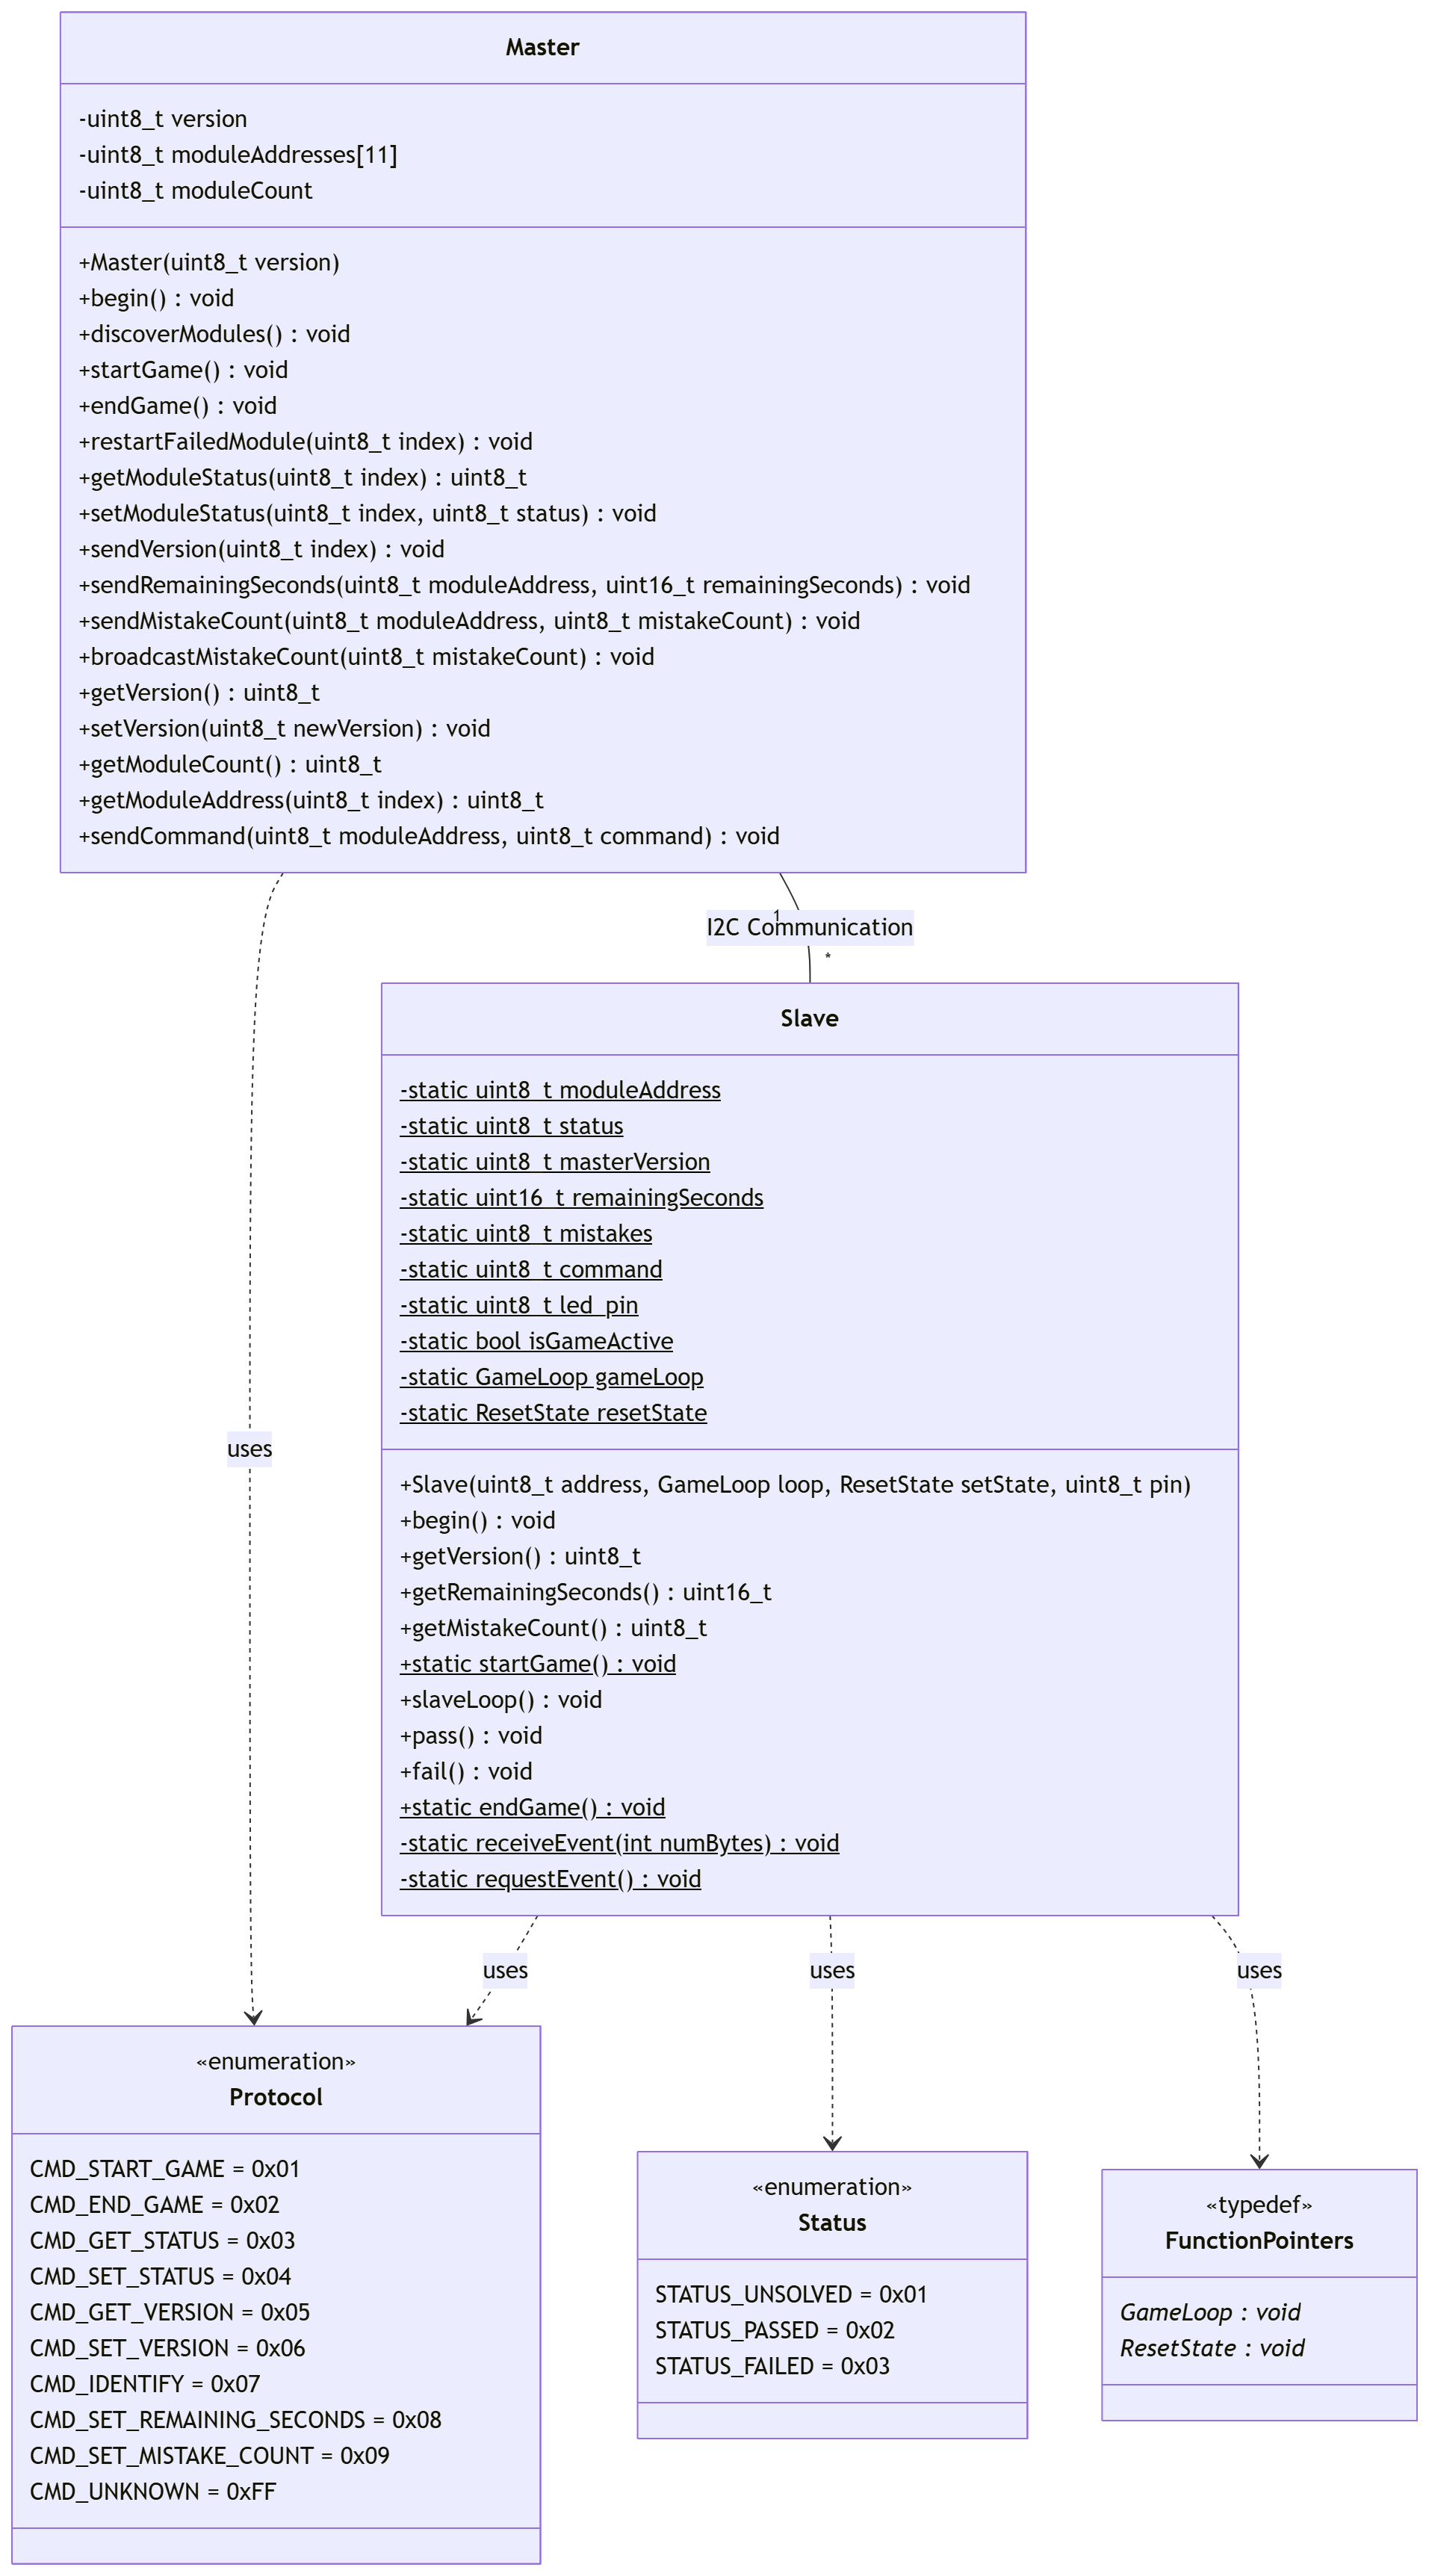
\includegraphics[width=0.85\textwidth]{diagram_klas.png}
  \caption{Diagram klas biblioteki ModuleComms --- relacja Master-Slave z protokołem komunikacyjnym (opracowanie własne)}
  \label{fig:class_modulecomms}
\end{figure}

Diagram klas przedstawia strukturę autorskiej biblioteki komunikacyjnej, w tym klasy \texttt{Master} (odpowiadającą za jednostkę nadrzędną) oraz \texttt{Slave} (reprezentującą podległe moduły), a także powiązane z nimi typy wyliczeniowe \texttt{Protocol} i \texttt{Status}. Implementacja wykorzystuje mechanizm wstrzykiwania funkcji zwrotnych (wskaźniki \texttt{GameLoop} i \texttt{ResetState}), co pozwala na pełną separację warstwy sieciowej od logiki biznesowej konkretnych zadań.
Metoda \texttt{getModuleStatus()} umożliwia odczyt stanu poszczególnych węzłów.

Klasa \texttt{Slave} reprezentuje stronę odbiorczą protokołu. Wykorzystuje statyczne pola i metody ze względu na ograniczenia biblioteki \texttt{Wire.h}, która wymaga rejestracji funkcji zwrotnych w postaci wskaźników na funkcje wolnostojące. Wstrzykiwanie logiki gry odbywa się przez wskaźniki funkcyjne \texttt{GameLoop} oraz \texttt{ResetState}, przekazywane w konstruktorze --- stanowi to realizację wzorca odwrócenia sterowania (ang. \textit{Inversion of Control}), umożliwiającą każdemu modułowi zagadki dostarczenie własnej implementacji pętli gry bez modyfikacji kodu biblioteki komunikacyjnej.

Typy wyliczeniowe \texttt{Protocol} oraz \texttt{Status} definiują zestaw jednobajtowych kodów operacyjnych (\textit{opcodes}) przesyłanych na magistrali I$^2$C, zapewniając jednoznaczną interpretację ramek komunikacyjnych po obu stronach łącza.


\subsection{Diagram klas modułów zagadek}

Każdy moduł zagadki w systemie stanowi niezależną jednostkę logiczną, integrowaną z magistralą komunikacyjną poprzez instancję klasy \texttt{Slave} z biblioteki \texttt{ModuleComms}. Diagram przedstawiony na Rysunku~\ref{fig:class_modules} ilustruje strukturę pięciu zaimplementowanych modułów wraz z ich wewnętrznymi typami danych.

\begin{figure}[H]
  \centering
  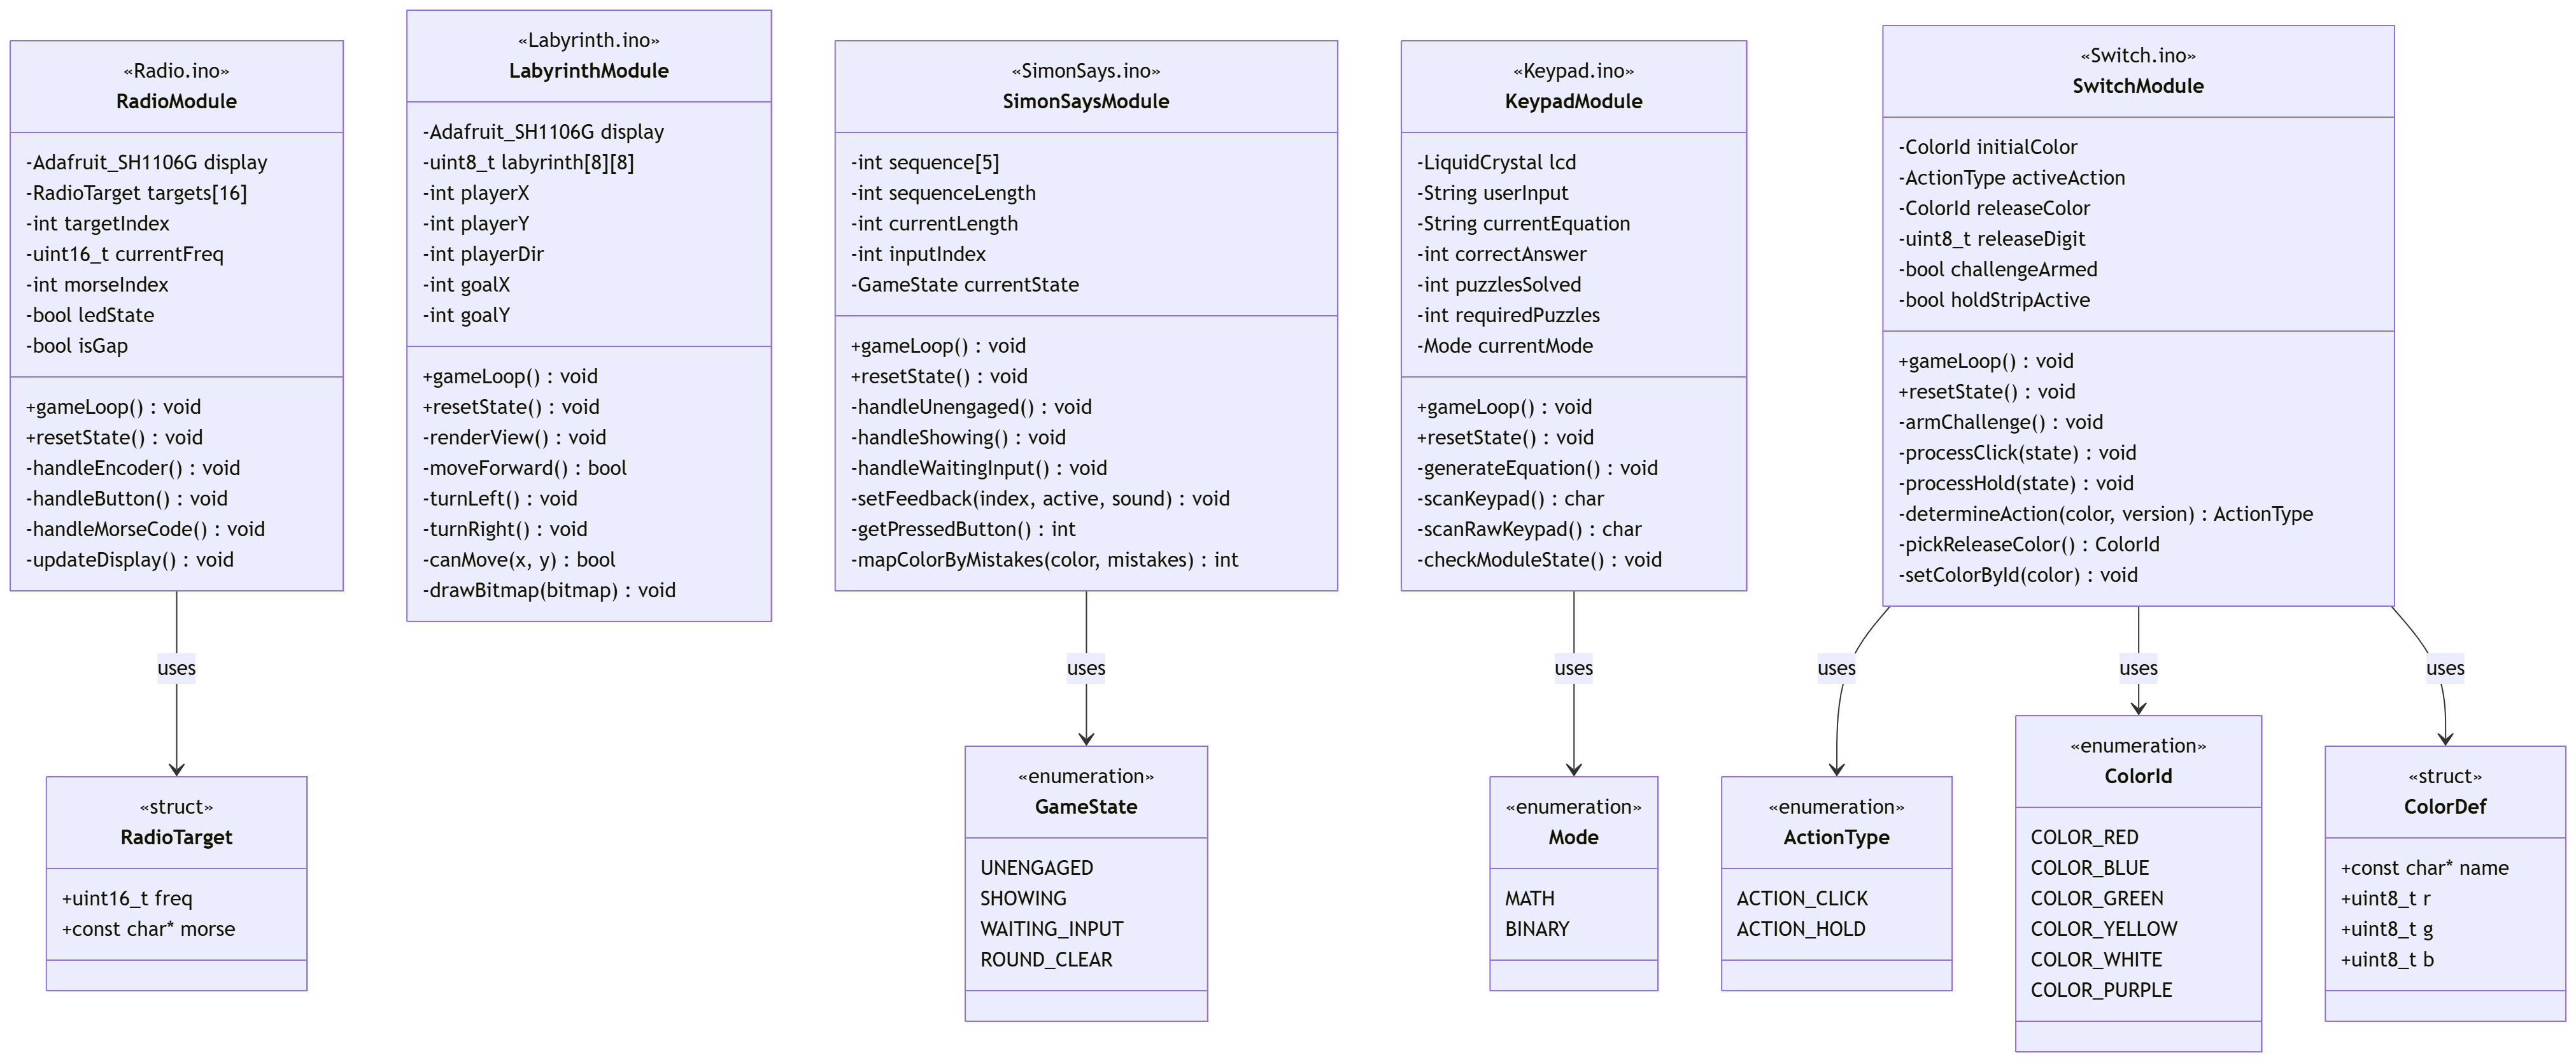
\includegraphics[width=0.95\textwidth]{diagram_klas_moduly.png}
  \caption{Diagram klas modułów zagadek z wewnętrznymi typami wyliczeniowymi i strukturami danych (opracowanie własne)}
  \label{fig:class_modules}
\end{figure}

Wspólnym elementem architektury wszystkich modułów jest mechanizm wstrzykiwania funkcji zwrotnych (ang. \textit{callbacks}) --- każdy moduł przekazuje w konstruktorze klasy \texttt{Slave} wskaźniki na swoje funkcje \texttt{gameLoop()} oraz \texttt{resetState()}, realizując wzorzec odwrócenia sterowania (ang. \textit{Inversion of Control}). Dzięki temu klasa \texttt{Slave} wywołuje logikę specyficzną dla danego modułu bez znajomości jej implementacji.

Moduły różnią się znacząco pod względem złożoności wewnętrznej. Moduł sekwencyjny wykorzystuje maszynę stanów (enum \texttt{GameState}) do zarządzania fazami rozgrywki, natomiast moduł z przełącznikiem operuje na typach wyliczeniowych \texttt{ActionType} i \texttt{ColorId} definiujących logikę decyzyjną opartą na kolorze diody RGB i numerze wersji gry. Moduł arytmetyczny implementuje dwa tryby pracy (enum \texttt{Mode}: arytmetyczny i binarny), a moduł radiowy przechowuje tablicę struktur \texttt{RadioTarget} z częstotliwościami i kodami Morse'a w pamięci Flash (\texttt{PROGMEM}).

\subsection{Diagram klas warstwy sprzętowej i bibliotek zewnętrznych}

Ostatni z diagramów (Rysunek~\ref{fig:class_libraries}) przedstawia mapę zależności pomiędzy modułami systemu a wykorzystywanymi bibliotekami zewnętrznymi. Diagram uwidacznia, w jaki sposób poszczególne węzły korzystają ze współdzielonych komponentów programowych.

\begin{figure}[H]
  \centering
  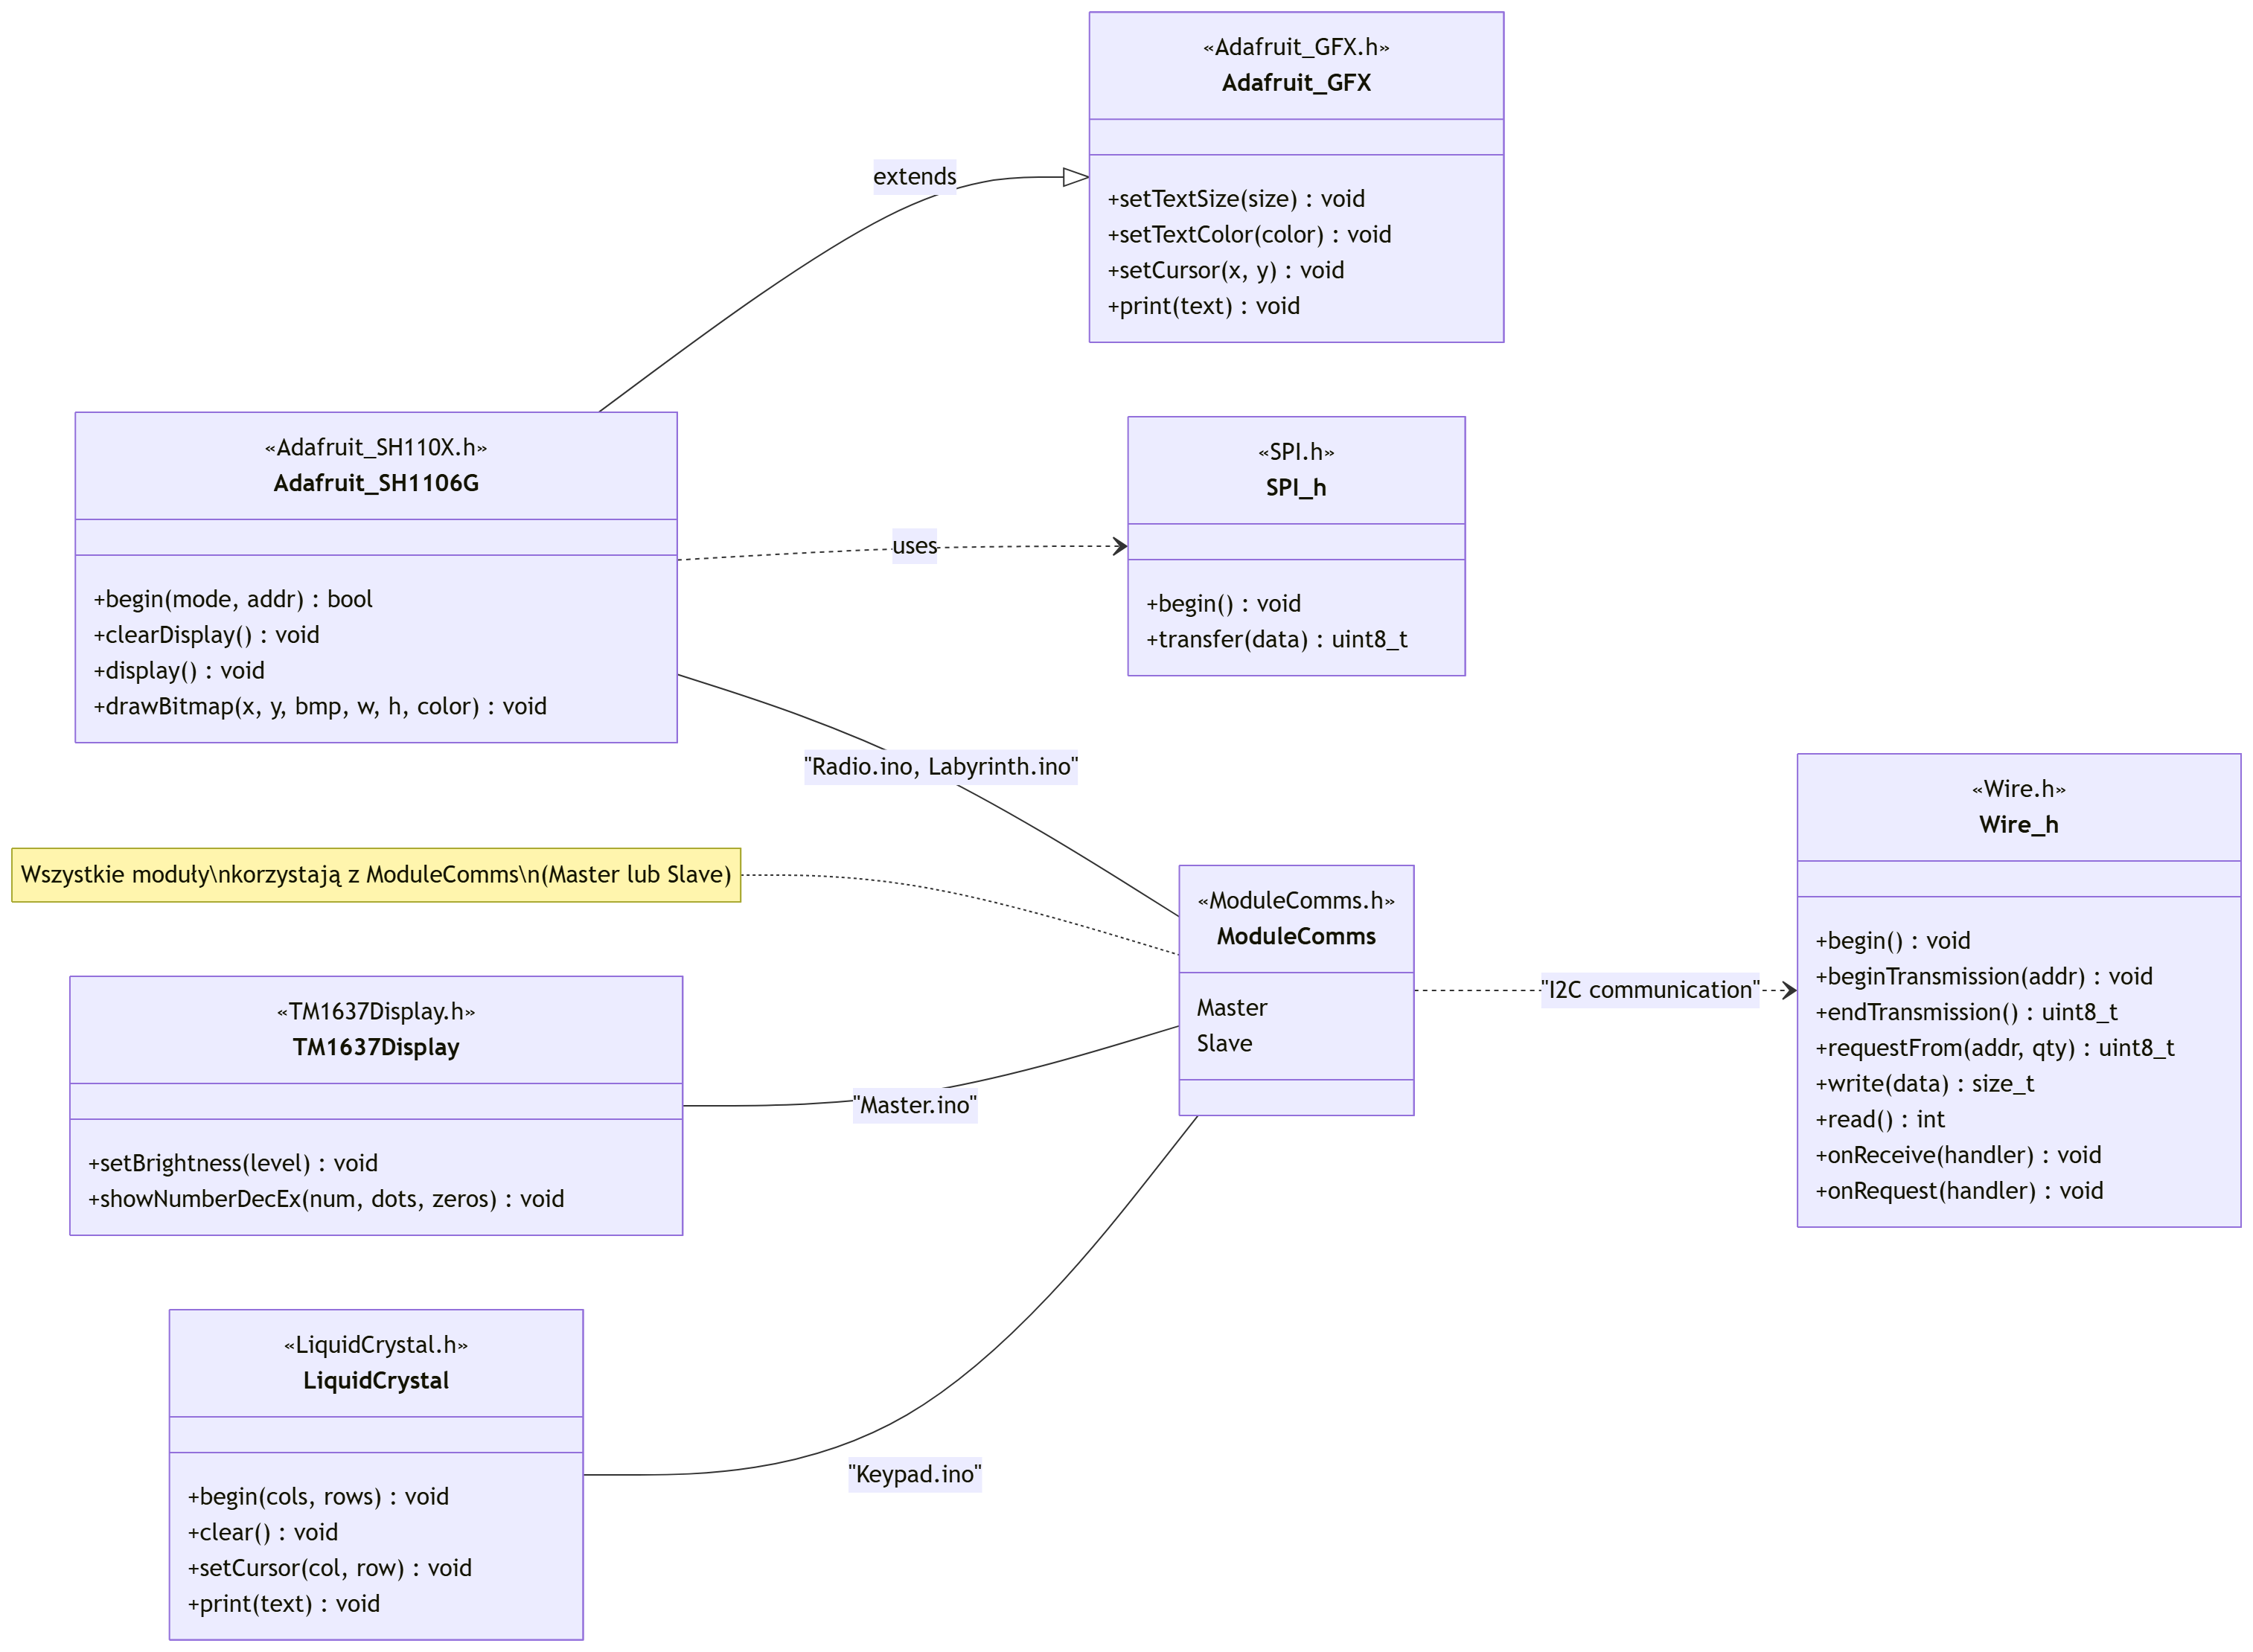
\includegraphics[width=0.95\textwidth]{diagram_klas_biblio.png}
  \caption{Diagram zależności warstwy sprzętowej --- powiązania modułów z bibliotekami zewnętrznymi (opracowanie własne)}
  \label{fig:class_libraries}
\end{figure}

Centralnym elementem jest biblioteka \texttt{ModuleComms}, z której korzystają wszystkie węzły systemu --- zarówno Master (klasa \texttt{Master}), jak i moduły zagadek (klasa \texttt{Slave}). Komunikacja realizowana jest za pośrednictwem biblioteki \texttt{Wire.h}, stanowiącej warstwę abstrakcji nad sprzętowym kontrolerem I$^2$C.

Moduły radiowy oraz labiryntu wykorzystują dodatkowo sterownik wyświetlaczy OLED \texttt{Adafruit\_SH1106G}, który dziedziczy po uniwersalnym rdzeniu graficznym \texttt{Adafruit\_GFX} i komunikuje się z wyświetlaczem przez interfejs SPI (\texttt{SPI.h}). Moduł arytmetyczny korzysta z biblioteki \texttt{LiquidCrystal} do obsługi panelu alfanumerycznego LCD, natomiast jednostka nadrzędna wykorzystuje \texttt{TM1637Display} do sterowania wyświetlaczem 7-segmentowym prezentującym czas rozgrywki. Moduł sekwencyjny oraz moduł z przełącznikiem nie wymagają zewnętrznych bibliotek peryferiów --- operują wyłącznie na pinach cyfrowych mikrokontrolera za pomocą standardowych funkcji Arduino.


\chapter{Implementacja}
W niniejszym rozdziale opisano praktyczną realizację założeń projektowych systemu. Nacisk położono na architekturę oprogramowania, implementację autorskiego protokołu komunikacyjnego, zastosowany wzorzec wielozadaniowości kooperatywnej oraz szczegółową budowę poszczególnych modułów zagadek. Dla każdego komponentu przedstawiono kluczowe fragmenty kodu źródłowego wraz z uzasadnieniem przyjętych rozwiązań programistycznych.

\section{Architektura oprogramowania}
Zaprojektowany system obwodu logiki gry operuje na płaszczyźnie architektury silnie rozproszonej z scentralizowanym panelem jednostki, definiując paradygmat jednego koordynującego serwera (\textit{Master}) nadzorującego liczne peryferyjne stanowiska obliczeniowe modułów (\textit{Slave}). Główną wytyczną podczas projektowania struktury oprogramowania procesorów było wdrożenie abstrakcji programowej dla logiki centrali, ujednolicającej wywołania stanu mikrokontrolerów pomimo skrajnych różnic stosowanych u nich fizycznych sensorów wykonawczych i różnorodności samych obwodów.

\section{Autorska biblioteka komunikacyjna ModuleComms}
Biblioteka \texttt{ModuleComms} powstała, aby ujednolicić obsługę komunikacji I$^2$C i uniknąć powielania kodu. Bez niej każdy moduł musiałby samodzielnie zarządzać buforowaniem danych i dekodowaniem ramek protokołu. Biblioteka przejmuje te zadania, oferując programiście gotowe funkcje do sprawdzania stanu modułów i obsługi logiki gry.

W protokole komunikacyjnym każde polecenie i każdy status to pojedynczy bajt. Komendy wywołujące akcję po stronie serwera to np. \texttt{CMD\_START\_GAME} czy \texttt{CMD\_IDENTIFY}, a flagi stanu modułu to \texttt{STATUS\_UNSOLVED}, \texttt{STATUS\_PASSED} i \texttt{STATUS\_FAILED}. Dzięki temu zamiast przesyłać przez magistralę pełne tekstowe identyfikatory poleceń wystarczy pojedynczy bajt --- co zmniejsza liczbę przesyłanych danych i zwiększa przepustowość komunikacji.
Listing~\ref{lst:modulecomms-protocol-defs} prezentuje komplet kodów komend i statusów używanych przez warstwę transportową biblioteki.
\begin{lstlisting}[language=C++, caption={Definicje protokołu transportowego I$^2$C w bibliotece ModuleComms}, label={lst:modulecomms-protocol-defs}]
#define CMD_START_GAME            0x01
#define CMD_END_GAME              0x02
#define CMD_GET_STATUS            0x03
#define CMD_SET_STATUS            0x04
#define CMD_GET_VERSION           0x05
#define CMD_SET_VERSION           0x06
#define CMD_IDENTIFY              0x07
#define CMD_SET_REMAINING_SECONDS 0x08
#define CMD_SET_MISTAKE_COUNT     0x09
#define CMD_UNKNOWN               0xFF

#define STATUS_UNSOLVED 0x01
#define STATUS_PASSED   0x02
#define STATUS_FAILED   0x03
\end{lstlisting}

Biblioteka udostępnia dwie główne klasy: \texttt{Master} --- dla jednostki nadrzędnej --- oraz \texttt{Slave} --- dla modułów podrzędnych.

Klasa \texttt{Master} odpowiada za koordynację systemu: skanuje magistralę w poszukiwaniu modułów (\texttt{discoverModules()}), przesyła pozostały czas gry (\texttt{sendRemainingSeconds()}) oraz rozgłasza liczbę błędów (\texttt{broadcastMistakeCount()}). Wykaz adresów modułów przechowywany jest w tablicy, co eliminuje potrzebę dynamicznej alokacji pamięci.

Listing~\ref{lst:modulecomms-master-interface} pokazuje publiczny interfejs klasy \texttt{Master}, odpowiedzialnej za orkiestrację rozgrywki.
\begin{lstlisting}[language=C++, caption={Interfejs główny platformy nadzorującej (ModuleComms.h)}, label={lst:modulecomms-master-interface}]
class Master {
public:
    Master(uint8_t version);
    void begin();
    void discoverModules();
    void startGame();
    void endGame();
    void restartFailedModule(uint8_t index);
    
    // Obieg stanu i propagacja zmiennych gry do wbudowanych zagadek
    uint8_t getModuleStatus(uint8_t index);
    void sendRemainingSeconds(uint8_t moduleAddress, uint16_t remainingSeconds);
    void broadcastMistakeCount(uint8_t mistakeCount);
    void sendCommand(uint8_t moduleAddress, uint8_t command);
private:
    uint8_t version;
    uint8_t moduleAddresses[11];
    uint8_t moduleCount;
};
\end{lstlisting}

Dzięki takiej architekturze \texttt{Master} nie musi znać szczegółów działania poszczególnych modułów. Każdy z nich jest traktowany jako „czarna skrzynka”, która zwraca jedynie informację o swoim stanie: sukces, błąd lub oczekiwanie.

Integracja modułu z biblioteką polega na przekazaniu dwóch funkcji: \texttt{gameLoopFn} (logika zagadki) oraz \texttt{resetStateFn} (powrót do stanu początkowego). Jest to realizacja wzorca odwrócenia sterowania (ang. \textit{Inversion of Control}) --- moduł dostarcza kod, a biblioteka decyduje o momencie jego wywołania. Programista musi jedynie wywołać \texttt{slave.slaveLoop()} w głównej pętli Arduino.

Listing~\ref{lst:modulecomms-slave-interface} zawiera uproszczony interfejs klasy \texttt{Slave} wraz z funkcjami zwrotnymi.
\begin{lstlisting}[language=C++, caption={Uproszczona definicja interfejsu polimorficznego do węzłów łamigłówek (ModuleComms.h)}, label={lst:modulecomms-slave-interface}]
typedef void (*GameLoop)();
typedef void (*ResetState)();

class Slave {
public:
    Slave(uint8_t address, GameLoop loop, ResetState setState, uint8_t pin);
    void begin();
    
    // Obsługa niewidocznych funkcji wejścia:
    void slaveLoop(); 

    // Publiczne emitery aktualizujące stan logiczny flag na maszynie stanów
    void pass();
    void fail();
    
    // Aktualizacje rozproszone przetrzymujące pozycję z serwera
    uint8_t getVersion();
    uint16_t getRemainingSeconds();
    uint8_t getMistakeCount();
private:
    static GameLoop gameLoop;
    static ResetState resetState;
    // Niskopoziomowy dostęp odczytu sprzętowego z podpięcia \texttt{Wire.h}
    static void receiveEvent(int numBytes);
    static void requestEvent();
};
\end{lstlisting}

Jednostka Master zarządza komunikacją poprzez cykliczne odpytywanie wszystkich modułów podłączonych do magistrali. Wykorzystuje do tego funkcję \texttt{Wire.requestFrom()}, która pozwala na pewne pobranie statusu z każdego węzła. Jeżeli moduł zgłosi stan \texttt{STATUS\_PASSED}, Master przestaje go odpytywać, uznając zadanie za wykonane. W przypadku zgłoszenia \texttt{STATUS\_FAILED}, licznik błędów systemu zostaje zwiększony. Po przekroczeniu dopuszczalnej liczby błędów lub upływie czasu, Master wysyła do wszystkich modułów sygnał zakończenia gry, co powoduje zablokowanie ich logiki i wywołanie funkcji resetującej stan urządzenia.

\section{Wielozadaniowość kooperatywna i wstrzymania nieblokujące}
Standardowe podejście w środowisku Arduino do odmierzania czasu opiera się na funkcji \texttt{delay()}. Skutkuje ona jednak zatrzymaniem pracy procesora na określony czas (ang. \textit{busy waiting}), co uniemożliwia wykonywanie innych zadań w tle. Ze względu na asynchroniczny model komunikacji I$^2$C stosowany w niniejszej pracy, użycie blokującego oczekiwania doprowadziłoby do utraty nadchodzących pakietów danych i żądań ze sterownika Master, co skutkowałoby błędami desynchronizacji (ang. \textit{timeout}).

Aby zagwarantować pełną responsywność systemu i uniknąć kolizji na magistrali, wdrożono wzorzec \textbf{wielozadaniowości kooperatywnej} (ang. \textit{cooperative multitasking}). Zamiast zatrzymywać program, wykorzystano nieblokujące liczniki programowe (ang. \textit{non-blocking software timers}) oparte na funkcji \texttt{millis()}. We wszystkich modułach główna pętla \texttt{loop()} wykonuje się nieustannie, a logika programu jedynie sprawdza, czy od ostatniego zdarzenia upłynął wymagany interwał czasowy. Pozwala to mikrokontrolerowi na jednoczesne odświeżanie wyświetlaczy, skanowanie przycisków oraz ciągłe nasłuchiwanie na magistrali I$^2$C bez ryzyka zablokowania komunikacji.

\section{Implementacja obwodów i modułów wbudowanych}
\subsection{Moduł nadrzędny}
Stacja nadrzędna stanowi centralny punkt decyzyjny całego omawianego systemu. Jako jedyna z peryferiów, nie implementuje ona podrzędnego interfejsu zagadek, lecz służy za główny zegar odliczający i dystrybutor globalnych ustawień gry. Stacja nadrzędna została rozbudowana o poczwórny wyświetlacz 7-segmentowy (\texttt{TM1637}), pełniący rolę głównego wskaźnika czasu, oraz dodatkowy, 2-cyfrowy wyświetlacz 7-segmentowy obsługiwany przez rejestry przesuwne. Ten drugi służy do prezentacji wylosowanego ziarna pseudolosowości (zmiennej \texttt{version}), determinującego logikę pozostałych modułów. Interfejs wyposażono również w przycisk Start, przełącznik dźwigniowy oraz przetwornik piezoelektryczny (buzzer) do sygnalizacji dźwiękowej.

Mikrokontroler reguluje tempo narastających ostrzeżeń dźwiękowych. Stabilność tego modułu opiera się na nieblokującej funkcji \texttt{handleBeeps()}, której algorytm wyznacza odstępy między sygnałami w oparciu o różnicę między pozostałym czasem gry a progiem krytycznym (\texttt{steadyBeepThreshold}). Gdy rezerwa czasu spadnie poniżej progu, sygnał staje się ciągły. Wykorzystano do tego wartość zmiennoprzecinkową \texttt{progress}, która estymuje wymagany sukcesywny spadek interwału \texttt{beepInterval}. Dzięki rezygnacji z instrukcji \texttt{delay()}, Master zachowuje pełną responsywność na pakiety przychodzące z magistrali I$^2$C.

Listing~\ref{lst:master-handlebeeps} przedstawia implementację funkcji \texttt{handleBeeps()}, która dynamicznie skraca interwał sygnałów ostrzegawczych.
\begin{lstlisting}[language=C++, caption={Nieblokująca obsługa przyspieszonego upływu czasu ostrzegawczego (Master.ino)}, label={lst:master-handlebeeps}]
void handleBeeps() {
  if (millis() - lastBeepTime >= beepInterval) {
    beep();
    lastBeepTime = millis();

    // Kalkulacja przyspieszania odstępów w miarę upływu czasu
    if (remainingTime > steadyBeepThreshold) {
      float progress = float(remainingTime - steadyBeepThreshold) 
                       / float(gameDurationSeconds - steadyBeepThreshold);
      beepInterval = finalInterval + (initialInterval - finalInterval) * progress;
    } else {
      beepInterval = finalInterval; // Sygnał ciągły po przekroczeniu progu
    }
  }
}
\end{lstlisting}

Ważnym elementem zabezpieczającym obsługę przełącznika jest funkcja \texttt{handle\allowbreak Switch()}. Aby zapobiec przypadkowemu przerwaniu rozgrywki, wdrożono mechanizm potwierdzenia resetu. Operator (wyłącznie w celach diagnostycznych) musi trzykrotnie przełączyć dźwignię w krótkim odstępie czasu, zdefiniowanym przez \texttt{SWITCH\_RESET\_TIMEOUT}, aby wywołać procedurę \texttt{resetGame()} i przywrócić system do stanu gotowości.

Listing~\ref{lst:master-handleswitch} ilustruje licznik okna czasowego używany do bezpiecznego potwierdzania resetu.
\begin{lstlisting}[language=C++, caption={Programowe ubezpieczenie przed przypadkowym restartem gry z licznikiem czasowym operacji (Master.ino)}, label={lst:master-handleswitch}]
void handleSwitch() {
  bool currentSwitchState = (digitalRead(SWITCH_PIN) == LOW);
  if (currentSwitchState != isSwitchOn) {
    isSwitchOn = currentSwitchState; // Detekcja przerzucenia prądu na przełączniku
    if (!isSwitchOn) { 
      unsigned long currentTime = millis();
      
      // Zliczanie prób na oknie resetów
      if (currentTime - lastSwitchOffTime < SWITCH_RESET_TIMEOUT) {
        switchOffCount++;
        if (switchOffCount >= 3) {
          resetGame(); // Resetowanie gry i powiadomienie modułów Slave
          switchOffCount = 0;
        }
      } else {
        switchOffCount = 1;
      }
      lastSwitchOffTime = currentTime;
    } else {
      if (!isGameInProgress) startGame();
    }
  }
}
\end{lstlisting}

Kluczowa dla przebiegu gry jest funkcja \texttt{checkModules()}, która odpowiada za sprawdzenie warunków zwycięstwa lub porażki. Master sekwencyjnie pobiera statusy ze wszystkich zarejestrowanych modułów (\texttt{STATUS\_PASSED}, \texttt{STATUS\_FAILED} lub \texttt{STATUS\_UNSOLVED}). Na tej podstawie system decyduje, czy cała zagadka została rozwiązana, czy też należy zarejestrować błąd popełniony przez graczy.

Listing~\ref{lst:master-checkmodules} pokazuje pętlę odpytywania modułów i priorytetowe przechwytywanie stanu błędu.
\begin{lstlisting}[language=C++, caption={Procedura odpytywania stacji na nasłuchu I$^2$C (Master.ino)}, label={lst:master-checkmodules}]
void checkModules() {
  areAllModulesSolved = true;
  failedModuleIndex = -1;
  for (uint8_t i = 0; i < master.getModuleCount(); i++) {
    uint8_t status = master.getModuleStatus(i);
    // Jedyna definicja sukcesu dla całego urządzenia: wszystkie zgłaszają PASS
    if (status != STATUS_PASSED) {
      areAllModulesSolved = false;
    }
    // Przechwytywanie błędu jako absolutny priorytet iteracji
    if (status == STATUS_FAILED) {
      failedModuleIndex = i;
      break;
    }
  }
}
\end{lstlisting}

Główna logika sterownika Master znajduje się w pętli \texttt{loop()}. Gdy gra trwa (\texttt{isGameInProgress}), system zarządza czterema kluczowymi zadaniami: odliczaniem czasu (\texttt{updateGameTimer()}), sygnalizacją dźwiękową (\texttt{handleBeeps()}), obsługą diody błędu (\texttt{handleMistakeBlinking()}) oraz cyklicznym sprawdzaniem statusu podłączonych urządzeń. Funkcja \texttt{handleMistakeBlinking()} informuje o liczbie błędów poprzez serię błyśnięć czerwonej diody LED powtarzaną co 5 sekund. W przypadku wykrycia awarii modułu, Master uruchamia procedurę \texttt{handleFailure()}, która sygnalizuje błąd dźwiękiem i resetuje dany moduł, pozwalając na ponowne rozwiązanie zagadki.

Listing~\ref{lst:master-main-loop} przedstawia kompletną pętlę główną jednostki nadrzędnej z podziałem na zadania cykliczne.
\begin{lstlisting}[language=C++, caption={Główna pętla sterująca jednostki nadrzędnej (Master.ino)}, label={lst:master-main-loop}]
void loop() {
  handleSwitch();   // Odczyt statusu zasilania/restartu
  handleButton();   // Manualne uruchomienie po starcie

  if (isGameEnded && !isSwitchOn) {
    resetGame();
    isGameEnded = false;
  }

  if (isGameInProgress) {
    updateGameTimer();
    handleBeeps();
    handleMistakeBlinking();

    if (isHandlingFailure) {
      handleFailure(); // Procedura pauzująca wymuszona błędnym stanem modułu
    } else {
      checkModules();  // Aktualizacja stanu wszystkich modułów
      checkWinLose();  // Weryfikacja warunków końca gry
    }

    delay(50); // Bufor mitygujący zapchanie magistrali I2C
  }
}
\end{lstlisting}


\subsection{Moduł radiowy} Stanowi łamigłówkę opartą na dekodowaniu alfabetu Morse'a i strojeniu częstotliwości radiowej. Na module prezentowany jest sygnał nawigacyjny w postaci migającej diody LED wysokiej jasności, odwzorowującej rytm kodu Morse'a. Zadaniem gracza jest odsłuchanie i rozkodowanie sekwencji sygnałów w celu ustalenia słowa kluczowego, a następnie odszukanie powiązanej z nim częstotliwości nadajnika w materiałach referencyjnych i wybranie jej za pomocą inkrementalnego enkodera obrotowego. Poprawne dostrojenie transpondera kończy zagadkę.

Koordynację wszystkich systemów modułu — odświeżania ekranu, obsługi enkodera oraz generowania sygnałów świetlnych — realizuje funkcja \texttt{gameLoop()}. Jest ona wywoływana asynchronicznie przez bibliotekę komunikacyjną, co pozwala na zachowanie responsywności węzła przy jednoczesnym wykonywaniu logiki gry.

Listing~\ref{lst:radio-gameloop} pokazuje kolejność wywołań funkcji odpowiedzialnych za logikę modułu radiowego.
\begin{lstlisting}[language=C++, caption={Główna pętla logiczna modułu radiowego (Radio.ino)}, label={lst:radio-gameloop}]
void gameLoop() {
    // Pierwszorzędne odświeżenie ekranu po inicjalizacji gry
    if (needsInitialRender) {
        updateDisplay();
        needsInitialRender = false;
    }
    handleEncoder();    // Obsługa strojenia częstotliwości
    handleButton();     // Weryfikacja naciśnięcia przycisku zatwierdzenia
    handleMorseCode();  // Asynchroniczne generowanie kodu Morse'a na diodzie LED
}
\end{lstlisting}

Zastosowany model programowania opiera się na maszynie stanów i nieblokujących licznikach \texttt{millis()}, dzięki czemu animacja diody LED nie wstrzymuje pracy procesora. Kluczowym wyzwaniem implementacyjnym była optymalizacja pamięci SRAM, na którą duży wpływ ma sterownik wyświetlacza OLED (rezerwujący dynamicznie 1024 bajty na bufor ramki). Aby uniknąć przepełnienia stosu, wszystkie definicje słów i częstotliwości zostały przeniesione do nieulotnej pamięci programu.

Listing~\ref{lst:radio-progmem-targets} prezentuje strukturę danych \texttt{RadioTarget} oraz deklaracje \texttt{PROGMEM} użyte do oszczędzania pamięci SRAM.
\begin{lstlisting}[language=C++, caption={Deklaracja haseł telegraficznych i częstotliwości w pamięci Flash (Radio.ino)}, label={lst:radio-progmem-targets}]
const char m_0[] PROGMEM = "... .... . .-.. .-..";
// [...]
const char m_15[] PROGMEM = "-... . .- - ...";

struct RadioTarget {
    uint16_t freq;      // Częstotliwość docelowa nadajnika (np. 3505 dla 3.505 MHz)
    const char* morse;  // Wskaźnik do ciągu znaków w pamięci Flash
};

const RadioTarget targets[] = {
    {3505, m_0},        // shell
    // [...]
    {3608, m_15}        // beats
};
\end{lstlisting}

\subsection{Moduł labiryntu} Stanowi przestrzenną łamigłówkę nawigacyjną, w której gracz porusza się wewnątrz wirtualnego labiryntu za pomocą trzech przycisków (ruch na wprost oraz obroty w prawo lub w lewo). Interfejs graficzny oparto na wyświetlaczu OLED 128x64 pikseli. Co istotne, w przeciwieństwie do innych modułów, system ten komunikuje się z ekranem za pomocą szybkiej magistrali SPI (piny \texttt{MOSI}, \texttt{CLK}, \texttt{CS}, \texttt{DC}, \texttt{RST}). Wybór tego standardu zamiast I$^2$C podyktowany był nie tylko wyższą przepustowością niezbędną do odświeżania pełnoekranowych bitmap, ale przede wszystkim ograniczeniem sprzętowym mikrokontrolera. ATmega328P posiada tylko jeden interfejs I$^2$C, który w tym przypadku musi stale pracować w trybie Slave, by odbierać komendy od Mastera. Równoczesne pełnienie roli Mastera dla wyświetlacza byłoby na tym układzie praktycznie niemożliwe.

Logika modułu opiera się na współdzieleniu funkcji \texttt{canMove()} zarówno do walidacji przemieszczeń gracza, jak i do dynamicznego generowania rzutu perspektywicznego. Sercem koordynacji jest funkcja \texttt{gameLoop()}, która w sposób nieblokujący zarządza stanem wejść i wyjść.

Listing~\ref{lst:labyrinth-gameloop} przedstawia nieblokującą obsługę wejść użytkownika i renderowania widoku labiryntu.
\begin{lstlisting}[language=C++, caption={Główna pętla logiczna modułu labiryntu (Labyrinth.ino)}, label={lst:labyrinth-gameloop}]
void gameLoop() {
  // Pierwszorzędne narysowanie widoku po starcie gry
  if (needsInitialRender) {
    renderView();
    needsInitialRender = false;
  }
  // Odczyt stanów przycisków sterujących
  bool btnLeft    = digitalRead(BTN_LEFT);
  bool btnForward = digitalRead(BTN_FORWARD);
  bool btnRight   = digitalRead(BTN_RIGHT);
  
  unsigned long currentMillis = millis();

  // Obsługa wejścia z programowym debouncingiem
  if (currentMillis - lastInputTime >= INPUT_DELAY) {
    if (!btnForward && lastBtnForward) {
      lastInputTime = currentMillis;
      if (moveForward()) {
        display.clearDisplay(); // Czyszczenie po wygranej
        display.display();
        return;
      }
      renderView();
    }
    else if (!btnLeft && lastBtnLeft) {
      lastInputTime = currentMillis;
      turnLeft();
      renderView();
    }
    else if (!btnRight && lastBtnRight) {
      lastInputTime = currentMillis;
      turnRight();
      renderView();
    }
  }
  // Zapamiętanie stanów do detekcji zbocza
  lastBtnLeft    = btnLeft;
  lastBtnForward = btnForward;
  lastBtnRight   = btnRight;
}
\end{lstlisting}

Warstwa wizualna budowana jest z przeskalowanych bitmap definiujących ściany w różnej odległości i perspektywie. Wszystkie elementy graficzne (np. \texttt{epd\_bitmap\_closed\_left\_far}) przechowywane są w pamięci Flash za pomocą dyrektywy \texttt{PROGMEM}. Każda bitmapa o wymiarach 128x64 piksele zajmuje 1024 bajty (1\,KB) pamięci nieulotnej, gdzie pojedynczy bajt definiuje stan ośmiu sąsiednich pikseli w poziomie. Dzięki takiemu podejściu, mimo że zbiór grafik waży aż 15\,KB, moduł mieści się w pamięci ATmega328P, rezerwując jedynie niezbędny stały bufor ramki (1\,KB) w pamięci operacyjnej SRAM. Moduł zajmuje 28234 bajty (87\%) Flash oraz 792 bajty (38\%) SRAM.


\subsection{Moduł sekwencyjny} Stanowi implementację klasycznej łamigłówki typu \textit{Simon Mówi}, w której gracz musi zapamiętać i bezbłędnie odwzorować rosnącą sekwencję sygnałów świetlno-dźwiękowych. Warstwa sprzętowa modułu opiera się na czterech przyciskach mechanicznych przypisanych do kolorów oraz przetworniku piezoelektrycznym. Przebieg rozgrywki podzielono na fazy prezentacji (\texttt{SHOWING}) oraz oczekiwania na wejście (\texttt{WAITING\_INPUT}), zarządzane przez maszynę stanów.

Kluczowym mechanizmem utrudniającym zadanie jest dynamiczne przypisywanie kolorów przycisków w zależności od aktualnej liczby błędów popełnionych w całej grze. Funkcja \texttt{mapColorByMistakes()} sprawia, że ten sam kolor sygnału może wymagać naciśnięcia innego przycisku w miarę narastania presji czasu i liczby pomyłek przesyłanych magistralą I$^2$C.

Koordynacja stanów gry odbywa się wewnątrz funkcji \texttt{gameLoop()}, która w każdym cyklu procesora sprawdza aktualny etap rozgrywki i wywołuje odpowiednie procedury obsługi prezentacji sekwencji lub odczytu wejść.

Listing~\ref{lst:simon-gameloop} ilustruje przejścia maszyny stanów pomiędzy fazami rundy modułu sekwencyjnego.
\begin{lstlisting}[language=C++, caption={Główna pętla logiczna modułu sekwencyjnego (SimonSays.ino)}, label={lst:simon-gameloop}]
void gameLoop() {
    switch (currentState) {
        case UNENGAGED:    handleUnengaged();    break;
        case SHOWING:      handleShowing();      break;
        case WAITING_INPUT: handleWaitingInput(); break;
        case ROUND_CLEAR: 
            if (millis() - stateTimer >= WAIT_AFTER_CORRECT) {
                showIndex = 0;
                inputIndex = 0; 
                currentState = SHOWING;
                stateTimer = millis();
            }
            break;
    }
}
\end{lstlisting}

Implementacja ta pozwala na zachowanie ciągłej łączności z jednostką Master przy jednoczesnej obsłudze animacji diod oraz sygnałów dźwiękowych.

Listing~\ref{lst:simon-mapcolor} pokazuje reguły mapowania kolorów przycisków zależnie od liczby błędów globalnych.
\begin{lstlisting}[language=C++, caption={Dynamiczne przypisywanie układu klawiszy w zależności od liczby błędów (SimonSays.ino)}, label={lst:simon-mapcolor}]
int mapColorByMistakes(int shownColor, uint8_t mistakeCount) {
    if (shownColor < 0 || shownColor > 3) return shownColor;

    if (mistakeCount == 0) {
        const int map0[4] = {BLUE, RED, GREEN, YELLOW};
        return map0[shownColor];
    }
    if (mistakeCount == 1) {
        const int map1[4] = {YELLOW, GREEN, BLUE, RED};
        return map1[shownColor];
    }
    const int map2plus[4] = {GREEN, YELLOW, RED, BLUE};
    return map2plus[shownColor];
}
\end{lstlisting}


\subsection{Moduł arytmetyczny} Stanowi łamigłówkę matematyczną, w której zadaniem gracza jest rozwiązanie proceduralnie generowanego zadania i wprowadzenie wyniku za pomocą klawiatury. Warstwa sprzętowa modułu składa się z 16-klawiszowej klawiaturze membranowej w topologii matrycowej oraz alfanumerycznego wyświetlacza LCD 16x2. W przeciwieństwie do założeń wykorzystujących adapter I$^2$C, w ostatecznej implementacji zdecydowano się na bezpośrednie sterowanie równoległe (6 linii sterujących), co pozwoliło na uproszczenie warstwy programowej kosztem wykorzystania większej liczby pinów mikrokontrolera (od D11 do A2).

Główna pętla gry \texttt{gameLoop()} zarządza stanem wyświetlacza, czasem oczekiwania po błędzie oraz interpretacją wejść z klawiatury.

Listing~\ref{lst:keypad-gameloop} przedstawia przebieg pętli głównej modułu arytmetycznego wraz z kontrolą pauzy po błędzie.
\begin{lstlisting}[language=C++, caption={Główna pętla logiczna modułu arytmetycznego (Keypad.ino)}, label={lst:keypad-gameloop}]
void gameLoop() {
  // Obsługa wymuszonej pauzy po popełnieniu błędu
  if (waitingAfterMistake) {
    if (millis() >= nextEquationAt) {
      waitingAfterMistake = false;
      generateEquation();
    } else {
      return;
    }
  }
  // Odświeżenie interfejsu przy zmianie zadania
  if (updateDisplay) {
    lcd.clear();
    lcdPrintLine(0, (currentMode == BINARY) ? lastBinary : currentEquation);
    updateDisplay = false;
  }
  // Skanowanie wejść od gracza
  char key = scanKeypad();
  if (key != '\0') {
    handleKey(key); // Rozpoznawanie liczb i znaków funkcyjnych
  }
}
\end{lstlisting}

Algorytm generuje zadania w dwóch trybach (ustalanych na podstawie globalnej zmiennej \texttt{version}): arytmetycznym (podstawowe działania matematyczne) oraz binarnym (konwersja liczb dziesiętnych na binarne). Wdrożenie obsługi wejścia wymagało precyzyjnego mechanizmu eliminowania drgań styków (ang. \textit{debouncing}), aby uniknąć rejestrowania wielokrotnych naciśnięć tego samego klawisza.

Listing~\ref{lst:keypad-scankeypad} zawiera implementację programowego debouncera dla matrycy klawiatury.
\begin{lstlisting}[language=C++, caption={Nieblokujący odczyt klawiatury z programowym debouncingiem (Keypad.ino)}, label={lst:keypad-scankeypad}]
char scanKeypad() {
  char rawKey = scanRawKeypad(); // Odczyt sprzętowy matrycy
  unsigned long now = millis();

  // Detekcja zmiany stanu klawisza
  if (rawKey != lastRawKey) {
    lastRawKey = rawKey;
    keyLastChangeAt = now;
  }

  // Filtrowanie drgań styków (ignorowanie szybkich oscylacji)
  if (now - keyLastChangeAt < KEYPAD_DEBOUNCE_MS) {
    return '\0';
  }

  // Rejestracja stabilnego wciśnięcia
  if (rawKey != debouncedKey) {
    debouncedKey = rawKey;
    if (debouncedKey == '\0') {
      keyReported = false; // Reset po puszczeniu klawisza
    }
  }

  // Jednorazowe zgłoszenie naciśnięcia do logiki gry
  if (debouncedKey != '\0' && !keyReported) {
    keyReported = true;
    return debouncedKey;
  }
  return '\0';
}
\end{lstlisting}

\subsection{Moduł z przełącznikiem} Stanowi prostą, lecz wymagającą precyzji zagadkę, w której zadaniem gracza jest wykonanie właściwej akcji na fizycznym przełączniku dźwigniowym w oparciu o aktualny kolor podświetlenia diody RGB. W zależności od koloru i numeru wersji rozgrywki (\texttt{version}), moduł oczekuje jednej z dwóch akcji: szybkiego przełączenia (\textit{Click}) lub przytrzymania przełącznika (\textit{Hold}) do momentu wystąpienia konkretnej cyfry na liczniku głównym.

Koordynację stanów modułu realizuje funkcja \texttt{gameLoop()}, która monitoruje fizyczny stan pinu wejściowego i w zależności od wybranego trybu wywołuje procedury przetwarzające czas trwania interakcji.

Listing~\ref{lst:switch-gameloop} przedstawia logikę wyboru procedury \textit{Click}/\textit{Hold} w pętli modułu z przełącznikiem.
\begin{lstlisting}[language=C++, caption={Główna pętla logiczna modułu z przełącznikiem (Switch.ino)}, label={lst:switch-gameloop}]
void gameLoop() {
  // Inicjalizacja wyzwania przy starcie lub po resecie
  if (!challengeArmed) {
    armChallenge();
    return;
  }

  int currentState = digitalRead(SWITCH_PIN);

  // Wybór procedury weryfikacji w zależności od trybu
  if (activeAction == ACTION_CLICK) {
    processClick(currentState);
  } else {
    processHold(currentState);
  }
}
\end{lstlisting}

W przypadku akcji \textit{Hold}, dioda RGB zmienia kolor w momencie aktywacji przełącznika, podpowiadając graczowi moment zwolnienia dźwigni. Użytkownik musi puścić przełącznik w chwili, gdy ostatnia cyfra odliczanego przez Mastera czasu gry zgadza się z wartością przypisaną do danego koloru (np. cyfra 4 dla koloru niebieskiego).

Listing~\ref{lst:switch-determineaction} pokazuje reguły decyzyjne przypisujące akcję do kombinacji koloru i wersji rozgrywki.
\begin{lstlisting}[language=C++, caption={Wyznaczanie poprawnej procedury działania w oparciu o stan gry (Switch.ino)}, label={lst:switch-determineaction}]
ActionType determineAction(ColorId color, uint8_t version) {
    if (color == COLOR_GREEN) return ACTION_CLICK;

    // Logika warunkowa oparta na parzystości wersji
    if ((color == COLOR_RED || color == COLOR_BLUE) && (version % 2 == 0)) {
        return ACTION_CLICK;
    }
    if ((color == COLOR_BLUE || color == COLOR_YELLOW) && (version % 3 == 0)) {
        return ACTION_HOLD;
    }
    if (color == COLOR_YELLOW && (version % 2 == 0) && (version % 3 == 0)) {
        return ACTION_CLICK;
    }
    return ACTION_HOLD; // Domyślnie wymagane przytrzymanie
}
\end{lstlisting}

\chapter{Testy i działanie systemu}
Celem testów było sprawdzenie poprawności komunikacji I$^2$C, niezawodności logiki modułów oraz efektywności wykorzystania pamięci mikrokontrolerów ATmega328P. Analiza wyników potwierdziła spełnienie wymagań funkcjonalnych i niefunkcjonalnych.

Specyfika mikrokontrolerów AVR wymusza inną metodę testowania niż w przypadku komputerów PC. Podstawową weryfikacją jest pomyślna kompilacja kodu (\texttt{avr-gcc}), która sprawdza nie tylko składnię, ale i zajętość pamięci Flash oraz SRAM. Raporty kompilatora pozwalają upewnić się, że program mieści się w restrykcyjnych limitach sprzętowych.

Dodatkowym narzędziem diagnostycznym wykorzystywanym podczas prac nad prototypem była płytka Arduino Uno R4 WiFi, pełniąca rolę przekaźnika UART-USB. Ze względu na to, że programowane mikrokontrolery ATmega328P nie posiadały własnego połączenia szeregowego z komputerem (programowanie odbywało się przez programator ISP USBasp), do podglądu komunikatów diagnostycznych w czasie rzeczywistym podłączano linie TX/RX testowanego modułu do pinów płytki Arduino Uno R4, która przekazywała dane do komputera PC przez port szeregowy z prędkością 9600 baud. Umożliwiło to monitorowanie stanów wewnętrznych programu (m.in. wykrytych adresów I$^2$C, statusów modułów, wartości timerów) bez ingerencji w działanie systemu.

Uzupełnieniem weryfikacji kompilacyjnej były testy integracyjne przeprowadzone na fizycznym prototypie systemu:
\begin{itemize}
  \item \textbf{Walidacja wydajności kanału I$^2$C:} Testy z udziałem wszystkich 5 modułów Slave przy taktowaniu 100\,kHz potwierdziły stabilność komunikacji. Sekwencyjne odpytywanie przez jednostkę Master nie powodowało utraty danych ani błędów w przesyłanych ramkach protokołu \texttt{ModuleComms}.
  \item \textbf{Pomiar zużycia pamięci:} Wykorzystanie pamięci Flash i SRAM utrzymano na bezpiecznym poziomie dzięki alokacji danych statycznych w pamięci programu (dyrektywa \texttt{PROGMEM}).
\end{itemize}

\section{Analiza wykorzystania zasobów sprzętowych}
Wybór 8-bitowego mikrokontrolera ATmega328P jako platformy bazowej narzucił rygorystyczne wymagania dotyczące optymalizacji kodu. Poniższa tabela (Tabela~\ref{tab:memory_usage_summary}) zestawia ostateczne wyniki kompilacji dla wszystkich komponentów systemu, obrazując stopień wykorzystania dostępnej pamięci Flash oraz SRAM.

\begin{longtable}{|l|r|r|r|r|}
  \caption{Zestawienie wykorzystania pamięci mikrokontrolerów ATmega328P} \label{tab:memory_usage_summary}   \\
  \hline
  \textbf{Moduł}         & \textbf{Flash [B]} & \textbf{Flash [\%]} & \textbf{SRAM [B]} & \textbf{SRAM [\%]} \\
  \hline
  \endfirsthead

  \multicolumn{5}{c}%
  {{\bfseries Tabela \thetable{} -- kontynuacja z poprzedniej strony}}                                       \\
  \hline
  \textbf{Moduł}         & \textbf{Flash [B]} & \textbf{Flash [\%]} & \textbf{SRAM [B]} & \textbf{SRAM [\%]} \\
  \hline
  \endhead

  \hline \multicolumn{5}{|r|}{{Kontynuacja na następnej stronie}}                                            \\ \hline
  \endfoot

  \hline
  \endlastfoot

  Moduł nadrzędny        & 10106              & 31\%                & 964               & 47\%               \\ \hline
  Moduł radiowy          & 15326              & 47\%                & 1716*             & 84\%               \\ \hline
  Moduł labiryntu        & 28234              & 87\%                & 1816*             & 89\%               \\ \hline
  Moduł sekwencyjny      & 7812               & 24\%                & 480               & 23\%               \\ \hline
  Moduł arytmetyczny     & 9344               & 28\%                & 692               & 33\%               \\ \hline
  Moduł z przełącznikiem & 5452               & 16\%                & 545               & 26\%               \\ \hline
\end{longtable}
\noindent
\footnotesize{* Wartość uwzględniająca 1024 bajty bufora ramki obrazu alokowanego dynamicznie w pamięci SRAM przez bibliotekę graficzną, niewidocznego w statystykach kompilacji.}
\normalsize
\vspace{1em}

Największe wyzwanie pod kątem zasobów Flash stanowił moduł labiryntu, co wynika z konieczności przechowywania licznych bitmap renderowanych w perspektywie 3D. Z kolei w przypadku pamięci SRAM kluczowym ograniczeniem okazała się obecność wyświetlaczy OLED w modułach radiowym oraz labiryntu. Powyższa analiza (Tabela~\ref{tab:memory_usage_summary}) uwzględnia fakt, że sterowniki graficzne (np. \texttt{Adafruit\_SH1106G}) rezerwują w czasie działania programu dodatkowy bufor ramki o rozmiarze 1024 bajtów (128x64 pikseli monochromatycznych). Ponieważ alokacja ta odbywa się dynamicznie wewnątrz klasy sterownika, nie jest ona raportowana przez kompilator jako stałe zużycie pamięci operacyjnej. W rzeczywistości, po doliczeniu tego bufora, moduł labiryntu operuje na granicy stabilności sprzętowej, wykorzystując blisko 90\% dostępnej pamięci SRAM (2\,KB), co wymusiło rezygnację z jakichkolwiek innych struktur dynamicznych i oparcie logiki wyłącznie na zmiennych lokalnych oraz stałych \texttt{PROGMEM}.

Warto również zauważyć, że relatywnie wysokie użycie pamięci Flash w module radiowym (47\%) wynika z przechowywania sekwencji alfabetu Morse'a w postaci czytelnych ciągów znaków (np. kropki i kreski jako typ danych \texttt{char}). Rozwiązanie to wybrano ze względu na przejrzystość kodu i łatwość wprowadzania zmian. W przypadku konieczności dalszej optymalizacji, zasoby te można by zredukować poprzez zastosowanie kodowania bitowego (bit-packing), gdzie każda kropka i kreska reprezentowana byłaby przez pojedynczy bit, jednak przy obecnej skali projektu nie było to wymagane.

\section{Wyniki działania prototypu}
Przeprowadzone testy potwierdziły poprawność przyjętych założeń projektowych. Zastosowanie wielozadaniowości kooperatywnej oraz maszyn stanów pozwoliło na płynne działanie logiki gry i bezbłędne rejestrowanie zdarzeń z przycisków i sensorów. Od strony sprzętowej, zastosowanie rezystorów podciągających oraz stabilnego zasilania 5\,V zapewniło niezawodną, dwukierunkową komunikację między jednostką Master a modułami Slave.


\chapter{Podsumowanie i wnioski}
Celem pracy było zaprojektowanie modularnego systemu zadań logicznych na mikrokontrolerach ATmega328P. Niniejsza praca potwierdziła, że architektura nadrzędno-podrzędna (ang. \textit{Master-Slave}) i magistrala I$^2$C pozwalają na stworzenie stabilnego i skalowalnego systemu. Oprogramowanie umożliwia koordynację wielu modułów przy zachowaniu płynności interfejsu.

Niniejsza praca wykazała znaczenie optymalizacji pamięci (2\,KB SRAM). Wykorzystanie pamięci Flash (\texttt{PROGMEM}) oraz lekkiego protokołu komunikacyjnego pozwoliło na realizację złożonych zadań bez przekraczania limitów sprzętowych.

Głównym wyzwaniem technicznym okazało się zapewnienie stabilności sygnału na magistrali przy jednoczesnym poborze prądu przez wyświetlacze i diody, co wymagało zastosowania odpowiedniego filtrowania i zasilania. W ramach dalszego rozwoju projektu planowane jest zastąpienie niektórych mikrokontrolerów ATmega328P układami ESP32. Pozwoliłoby to na wykorzystanie łączności Wi-Fi do zdalnego monitorowania stanu gry oraz przeniesienie części obliczeń do centralnego systemu zarządzającego symulacją.

\begin{thebibliography}{20}
  \bibitem{atmega328p_datasheet}
  Microchip Technology Inc.,
  \emph{ATmega328P 8-bit AVR Microcontroller Datasheet},  Specyfikacja techniczna (Datasheet), \url{https://ww1.microchip.com/downloads/en/DeviceDoc/Atmel-7810-Automotive-Microcontrollers-ATmega328P_Datasheet.pdf}.
  \bibitem{cpp_arduino_ref}
  Arduino,
  \emph{Arduino Language Reference (C++)},
  Dokumentacja języka i struktury programowania środowiska Arduino IDE, opartego o C/C++,
  \url{https://www.arduino.cc/reference/en/}.
  \bibitem{arduino_liquid_crystal}
  Arduino,
  \emph{LiquidCrystal Library - API Documentation},
  Biblioteka referencyjna obsługi wyświetlaczy alfanumerycznych LCD (standard HD44780),
  \url{https://www.arduino.cc/reference/en/libraries/liquidcrystal/}.
  \bibitem{arduino_wire}
  Arduino,
  \emph{Wire Library - API Documentation},
  Biblioteka referencyjna rdzenia sprzętowego komunikacji TWI/I\textsuperscript{2}C interfejsów standardu Arduino, \url{https://www.arduino.cc/reference/en/language/functions/communication/wire/}.
  \bibitem{Adafruit_sh1106x}
  Limor Fried, Adafruit Industries,
  \emph{Adafruit SH110X Library},
  Wersja 2.1.8, Zoptymalizowany dla modułów macierzy węzłów, \url{https://github.com/adafruit/Adafruit_SH110x}.
  \bibitem{Adafruit-GFX-Library}
  Adafruit Industries,
  \emph{Adafruit GFX Library},
  Rdzeń procedur rysowania struktur 2D w środowisku mikrokontrolerów dla ekranów LCD/OLED,
  \url{https://github.com/adafruit/Adafruit-GFX-Library}.
  \bibitem{TM1637Display}
  Avishay Orpaz,
  \emph{TM1637Display},
  Driver wyświetlaczy podłączanych po magistrali 2-wire.
  \url{https://github.com/avishorp/TM1637}.

  \bibitem{stroustrup_cpp}
  Stroustrup B.,
  \emph{Język C++. Kompendium wiedzy}, wyd. IV, Helion, Gliwice 2014,
  ISBN: 978-83-246-8770-1.

  \bibitem{meyers_effective_modern_cpp}
  Meyers S.,
  \emph{Skuteczny nowoczesny C++}, Wydawnictwo Promise, Warszawa 2015,
  ISBN: 978-83-7541-168-3.

  \bibitem{josuttis_cpp_stdlib}
  Josuttis N. M.,
  \emph{C++ Biblioteka standardowa. Podręcznik programisty}, wyd. II, Helion, Gliwice 2014.

  \bibitem{gof_design_patterns}
  Gamma E., Helm R., Johnson R., Vlissides J.,
  \emph{Wzorce projektowe. Elementy oprogramowania obiektowego wielokrotnego użytku}, WNT, Warszawa 2010.

  \bibitem{francuz_avr_c}
  Francuz T.,
  \emph{Język C dla mikrokontrolerów AVR. Od podstaw do zaawansowanych aplikacji}, wyd. II, Helion, Gliwice 2015.

  \bibitem{blum_exploring_arduino}
  Blum J.,
  \emph{Odkrywanie Arduino. Narzędzia i techniki inżynierii pełnej czaru}, Helion, Gliwice 2020,
  ISBN: 978-83-283-6923-8.

  \bibitem{ganssle_art_embedded}
  Ganssle J.,
  \emph{The Art of Designing Embedded Systems}, wyd. 2, Newnes, 2008,
  ISBN: 978-0750686396.

  \bibitem{kwasniewski_avr_praktyce}
  Kwaśniewski S.,
  \emph{Mikrokontrolery AVR w praktyce}, Wydawnictwo BTC, Warszawa 2011.
\end{thebibliography}

\listoffigures
\listoftables

\end{document}